\documentclass{article}
\usepackage{graphicx} 
\usepackage{float}
\usepackage{booktabs}
\usepackage{array}
\usepackage{arydshln}
\usepackage{siunitx}
\usepackage{hyperref}
\usepackage{cancel}
\usepackage{changepage}
\usepackage{placeins}
\usepackage{enumitem}
\usepackage{siunitx}

%\usepackage{showframe}
\usepackage{times}

\DeclareSIUnit{\atm}{atm}

\usepackage{tabularx}
\usepackage{amsmath, amssymb, amscd, MnSymbol, mathrsfs}
\usepackage{cellspace}
\usepackage{tikz}
\usetikzlibrary{calc, patterns, angles, quotes, decorations.markings, decorations.pathmorphing, hobby}
\usepackage{xfrac}

\usepackage{chemfig}
\usepackage{caption}
\usepackage{tcolorbox}
\usepackage{bm}
\usepackage{pdfpages}
\usepackage{empheq}
\usepackage{pgfplots}
\usepackage{pgfplotstable}
\usepackage{xstring}

\pgfplotsset{compat=1.18}
\usepackage[oldvoltagedirection]{circuitikz}
\usepackage{microtype}
\usepackage{tikz-3dplot}
\usepackage{textcomp}
% Custom commands
\newcommand{\vect}[1]{\boldsymbol{\mathbf{#1}}}
\newcolumntype{C}{>{\centering\arraybackslash}X}
\newcolumntype{M}[1]{>{\centering\arraybackslash}m{#1}}

\usetikzlibrary{external}
\tikzexternalize[prefix=figures/]

\newcommand\myfrac[2]{\sfrac{#1\mkern-1.2mu}{#2}}
\usepackage{xcolor}

% Define custom colors
\definecolor{darkblue}{rgb}{0.1,0.1,0.5} % A dark blue shade
\definecolor{formalshade}{rgb}{0.95,0.95,1} % A light blue shade for the background

% For the adjustwidth environment
\PassOptionsToPackage{strict}{changepage}
\usepackage{changepage}

% For formal definitions
\usepackage{framed}

\newcommand{\formalsource}{} % Initialize an empty macro to store the source text

\newenvironment{formal}[3][]{% Start of the environment
	\renewcommand{\formalsource}{#1}% Store the optional argument
	\def\FrameCommand{%
		\hspace{1pt}%
		{\color{#2}\vrule width 2pt}%
		{\color{#3}\vrule width 4pt}%
		\colorbox{#3}%
	}%
	\MakeFramed{\advance\hsize-\width\FrameRestore}%
	\noindent\hspace{-4.55pt}% Disable indenting the first paragraph
	\begin{adjustwidth}{}{7pt}%
		\vspace{2pt}%
	}%
	{%
		\vspace{4pt}%
		\ifx\formalsource\empty % Check if the source is empty
		\else
		\hfill{\footnotesize{\formalsource}}% Align source to the bottom-right
		\fi
	\end{adjustwidth}\endMakeFramed%
}


% Custom itemize list with images for positive and negative items
\newlist{gitemize}{itemize}{1} % Just one level for the list
\setlist[gitemize,1]{
	leftmargin=2.8em, % Adjust the margin for the list
	labelsep=1em % Control the space between the label and the list item
}

% Define checkmark and cross symbols for positive and negative items
\newcommand{\checkitem}{\raisebox{-0.25\height}{\includegraphics[width=0.4cm]{checkmark.png}}}
\newcommand{\crossitem}{\raisebox{-0.25\height}{\includegraphics[width=0.4cm]{cross.png}}}


\usepackage[left=0.8in,right=0.8in,top=0.5in,bottom=0.69in,includeheadfoot,letterpaper]{geometry}
\usepackage{fancyhdr}
\usepackage{graphicx}
\usepackage{tabularray}
\usepackage{varwidth} 


\newcommand{\wm}[2]{%
	\begin{minipage}{#1\textwidth}
		\centering
		#2
	\end{minipage}%
}

\pagestyle{fancy}
\fancyhf{}


\renewcommand{\headrulewidth}{0.4pt}
\renewcommand{\footrulewidth}{0.4pt}

\fancyhead[L]{\includegraphics[height=1.2cm]{images/Kingston_University_London_logo_200-tablet.png}}
\fancyhead[R]{EG4024 – ME – Fluid Mechanics and Thermodynamics}
\fancyfoot[C]{Department of Mechanical Engineering}
\fancyfoot[R]{\thepage}

\usepackage{scalerel}

\setlength{\headheight}{30pt}
\setlength{\footskip}{20pt}



\usepackage[export]{adjustbox}
\usepackage{tocloft}
\renewcommand{\cfttoctitlefont}{}
\renewcommand{\contentsname}{}
\renewcommand{\cftsecleader}{\cftdotfill{\cftdotsep}}

\setlength{\cftbeforesecskip}{0.5em}


\usepackage{xcolor}      % For color options
\usepackage{hyperref}    % For hyperlinks
\usepackage{xurl}        % For better URL handling
\hypersetup{
	colorlinks=true,
	linkcolor=blue!50!black,
	urlcolor=blue,       % Color for URLs
}


\usepackage{xcolor}
\definecolor{ChineseGold}{HTML}{C59401}
\definecolor{AmericanGold}{HTML}{D3AF37}
\definecolor{MetallicSunburst}{HTML}{A77C37}
\definecolor{GoldenBrown}{HTML}{996515}
\definecolor{DarkBrown}{HTML}{674222}
\definecolor{SkyBlue}{HTML}{87CEEB}      % Soft and bright
\definecolor{BabyBlue}{HTML}{89CFF0}     % Gentle, pastel-like
\definecolor{SteelBlue}{HTML}{4682B4}    % Rich but not overpowering
\definecolor{RoyalBlue}{HTML}{4169E1}    % Strong, slightly purplish
\definecolor{MidnightBlue}{HTML}{191970} % Almost black, deep navy
\definecolor{PrussianBlue}{HTML}{003153} % Very deep blue with a classic look



%Refer to the equation as \eqref{equation}.
\usepackage{caption}  % This package allows captioning outside of a float
\usepackage[export]{adjustbox}


\usetikzlibrary{patterns}

\usetikzlibrary{patterns.meta}

\usepackage[para]{footmisc} % Example of making footnotes run together in a paragraph
\definecolor{darkgreen}{rgb}{0.0, 0.5, 0.0}  % Darker green

\usepackage{datetime}

\usepackage{xcolor}
\usepackage{tcolorbox}

\usepackage{etoolbox}

\makeatletter
\def\tagform@#1{\maketag@@@{{Eq.~#1}}} % Adds "Eq." and makes it bold
\makeatother
\usepackage{listings}
\lstdefinestyle{mypythonstyle}{
	language=Python,
	basicstyle=\ttfamily,
	showstringspaces=false,
	breaklines=true,
	commentstyle=\color{green!60!black},  % Softer gray for comments
	stringstyle=\color{orange},  % Different color for strings
	backgroundcolor=\color{gray!3},  % Light gray for background
	tabsize=4,
	belowcaptionskip=10pt, % Adjust space below caption
	morekeywords={lambda}, % Add lambda to keywords
	keywordstyle=\bfseries\color{pink!50!red},
	keywordstyle=[2]\color{blue!80!black},  % Specific style for 'lambda'
	morecomment=[l]{//},  % For inline comments
	literate={~} {$\sim$}{1},  % Converts tilde to a symbol
}
\begin{document}
	
	\vspace*{\fill}
	\begin{center}
		\textbf{\Huge Laboratory Report}\\[10pt]
		\LARGE \textbf{Pressure}
	\end{center}
	\vspace*{\fill}
	
	\Large    
	\begin{tabular}{@{}l l l@{}}
		\textbf{Submitted by:} & Sakariye Abiikar & K2371673 \\
		& Alireza Alishahi & K2333243 \\
		& Naim Alrifai & K2459662 \\
		& Munachi J Atuegbu & K2463699 \\
		& Ehsan Haque & K2453799 \\
		& Abdul Mueed & K2454880 \\   
		& Abdelrahman Shehata & K2426523 \\   
		& Varley, Freddie & K2311322
	\end{tabular}
	
	\vspace*{\fill}
	
	\begin{tabular}{@{}l l@{}}
		\textbf{Key Dates:} & Date of practical: Wednesday 19$^{\text{th}}$ March, 2025 \\
		& Deadline: Tuesday 3$^{\text{rd}}$ April, 2025 \\
		& Last Updated: \today\, \currenttime\\
	\end{tabular}
	\vspace*{\fill}
	
	\large
	\newpage\noindent	\vspace*{-1em}
	
	\begin{center}
		\LARGE \textbf{Contribution Table}\\[3em]
	\end{center}	
	
	
	\begin{tblr}{
			colspec={Q[4cm]Q[4cm]Q[4cm]Q[3cm]},
			hlines,vlines,
			cells={valign=m,halign=c},
			rows={ht=4\baselineskip},
			row{1}={ht=1.5\baselineskip,font=\bfseries},
		}
		Student & Course & Contribution & Picture \\ 
		Sakariye Abiikar & Mechanical Engineering & ~ & \includegraphics[width=2cm,valign=c]{images/image(7).jpeg} \\ 
		Alireza Alishahi & Mechanical Engineering  & ~ & 
\includegraphics[width=2cm,valign=c]{images//profile.jpg} \\ 
		Naim Alrifai & Mechanical Engineering & ~ & 
\includegraphics[width=2cm,valign=c]{images/profile.jpg} \\ 
		Munachi J Atuegbu & Mechanical Engineering & ~  & 
\includegraphics[width=2cm,valign=c]{images//profile.jpg} \\ 
		Ehsan Haque & Mechanical Engineering & ~ & 
\includegraphics[width=2cm,valign=c]{images//profile.jpg} \\
		Abdul Mueed & Mechanical Engineering  & ~ & 
\includegraphics[width=2cm,valign=c]{images/profile.jpg} \\ 
		Abdelrahman Shehata & Mechanical Engineering  & ~ & 
\includegraphics[width=2cm,valign=c]{images/profile.jpg}\\
		Varley, Freddie & Mechanical Engineering & &  
\includegraphics[width=2cm,valign=c]{images/profile.jpg} 
	\end{tblr}
		\vspace*{\fill}
	
	\normalsize
	\newpage\newgeometry{top=0.2in,bottom=0.6in,left=0.8in,right=0.8in}
	\noindent\vspace{0em}
	\begin{center}
		\LARGE \textbf{Table of Contents}\\[-7em]
	\end{center}
	{
		\hypersetup{linkcolor=black}
		\tableofcontents
	}    
	
	
	\large\newpage\restoregeometry\vspace*{-20pt}
	
	\noindent
	
\section{Abstract}
In this experiment, we calibrated and compared the performance of multiple pressure-measuring devices, including two Bourdon gauges, a Budenberg pressure gauge and a Hg glass manometer, in tandem with a reference pressure calibrator (DPI-603 Portable Pressure Calibrator), which served as the baseline for pressure measurements and as the source of the applied pressure. The devices were connected to the DPI-603 Portable Pressure Calibrator, enabling us to apply both positive and negative pressures in increments of approximately $\pm$5 kPa. Through this process, we were able to get an exhaustive dataset that demonstrated notable differences in the pressure-measuring devices' performance. \textcolor{red!50!white}{[Placeholder breif results findings]}. These results highlighted the importance of selecting appropriate devices based on precision requirements and operating conditions, as well as the potential impact of human error in reading analog instruments like the Bourdon gauges and Hg manometer. 

	
	\newpage\vspace*{-20pt}

	\section{Introduction}
	In engineering and scientific applications, pressure measurement is essential, playing a critical role in fields such as fluid dynamics, meteorology, and industrial control. Over time, pressure-measuring instruments have evolved, from early liquid column manometers to modern mechanical and digital gauges, each designed to provide accurate measurements under varying conditions.\\[1em]
	A key distinction in pressure measurement is between \textbf{absolute} and \textbf{gauge} pressure \footnote{\textbf{Differential} pressure i decided to redact in the context of our lab though it would be among this list}.\\ 
	Absolute pressure is measured relative to a vacuum, while gauge pressure is measured relative to atmospheric pressure. This distinction influences the design and function of pressure-measuring devices.\\[1em]
	Historically, the invention of the Bourdon gauge by Eugène Bourdon in 1849 marked a significant advancement in pressure measurement. It provided a robust and reliable means of monitoring pressure in industrial settings, where durability and consistency were paramount. On the other hand, liquid column manometers, particularly those using mercury, have been essential in laboratory settings due to their precision in measuring small pressure differences.\\[1em]
	Despite the advantages of different pressure-measuring devices, each has limitations, such as calibration errors and environmental influences.\\[1em]
	Previous studies have highlighted various challenges and findings related to pressure measurement devices. For example, a study by Hodgkinson et al. (2020) found that the accuracy of home blood pressure monitors varied significantly, with validated monitors showing a higher pass rate in static pressure tests compared to unvalidated ones. This emphasizes the importance of validation and calibration in ensuring the accuracy of pressure-measuring devices.\\[1em]
	In this experiment, we aimed to evaluate the performance and accuracy of various pressure-measuring devices under controlled conditions, comparing their responses to varying pressure levels.

	
	\newpage\vspace*{-20pt}
	\section{Method \& Experimental Procedures}\label{Method_Experimental_Procedures}
	%We are first given a table to record our findings as shown:\footnote{We started of in the lab by doing the refrigerator but this is redacted as its not a part of this lab report, following this we did the pressure lab experiment.}

	\begin{figure}[H] 
			\centering 
		    \begin{tikzpicture}[auto,
			block/.style ={rectangle, draw=gray!70!black, thick, fill=white!94!black, text width=1em,align=center, rounded corners, minimum height=2em},
			block1/.style ={rectangle, draw=gray!70!black, thick, fill=white!94!black, text width=5em,align=center, rounded corners, minimum height=2em},
			line/.style ={draw, thick, -latex',shorten >=2pt},
			cloud/.style ={draw=red, thick, ellipse,fill=red!20,
				minimum height=1em}]
			\node[anchor=center] (image) at (-10,0) {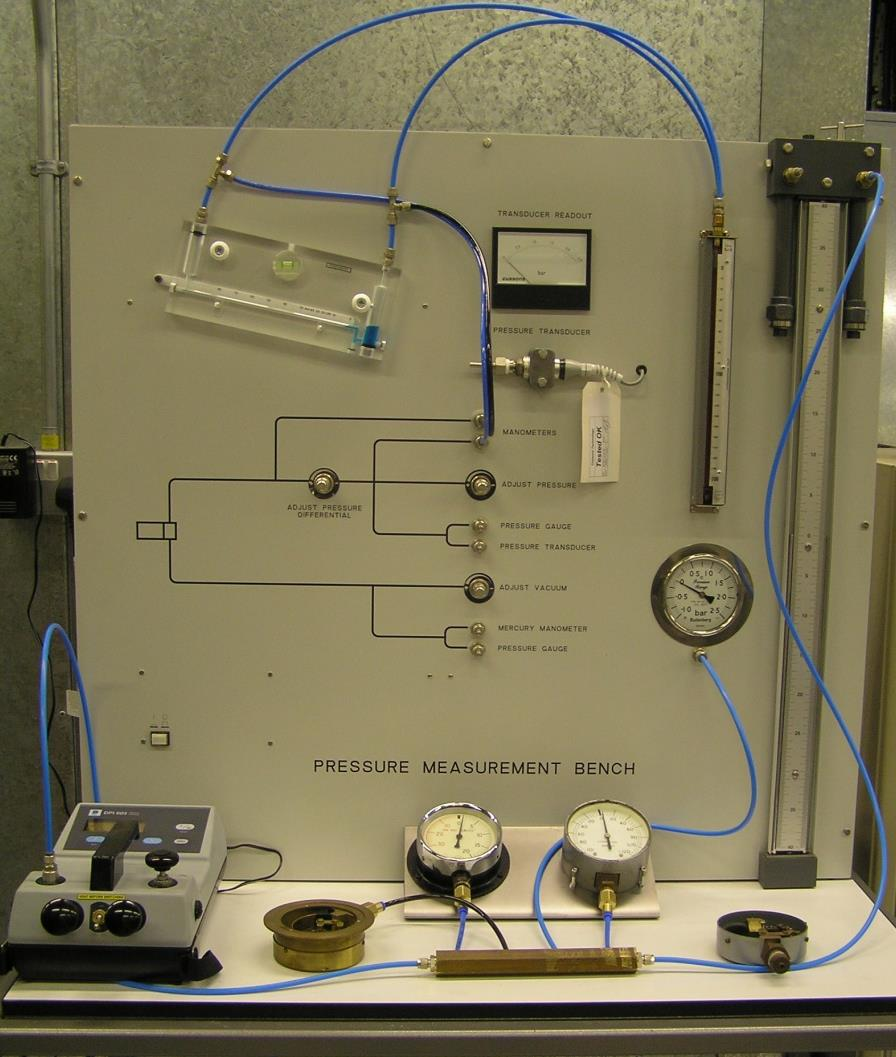
\includegraphics[width=0.9\textwidth]{extracted_images/image_7_1.png}};
			\node[block] (A) at (-9.85,-4.5) {1};
			\node[block] (B) at (-7.15,-4.5) {2};
			\node[block1] (Gauge) at (-8.5,-3.5) {Bourdon Gauge};
			%\draw[line] (Gauge.south) -- ++(0,-0.25) -| (A.north);
			%\draw[line] (Gauge.south) -- ++(0,-0.25) -| (B.north);			
			\node[block1] (Gauge) at (-15.5,-4.2) {Pressure calibrator};
			\node[block1] (Gauge) at (-7.5,-1.1) {Pressure Gauge};
			\node[block1] (Gauge) at (-3.5,7.6) {Mercury Glass Manometer};
		\end{tikzpicture}
		\caption{Pressure Measurement Bench} 
		\label{fig:pressure_measurement_bench} 
	\end{figure}
	
	\begin{figure}[H] 
			\centering 
			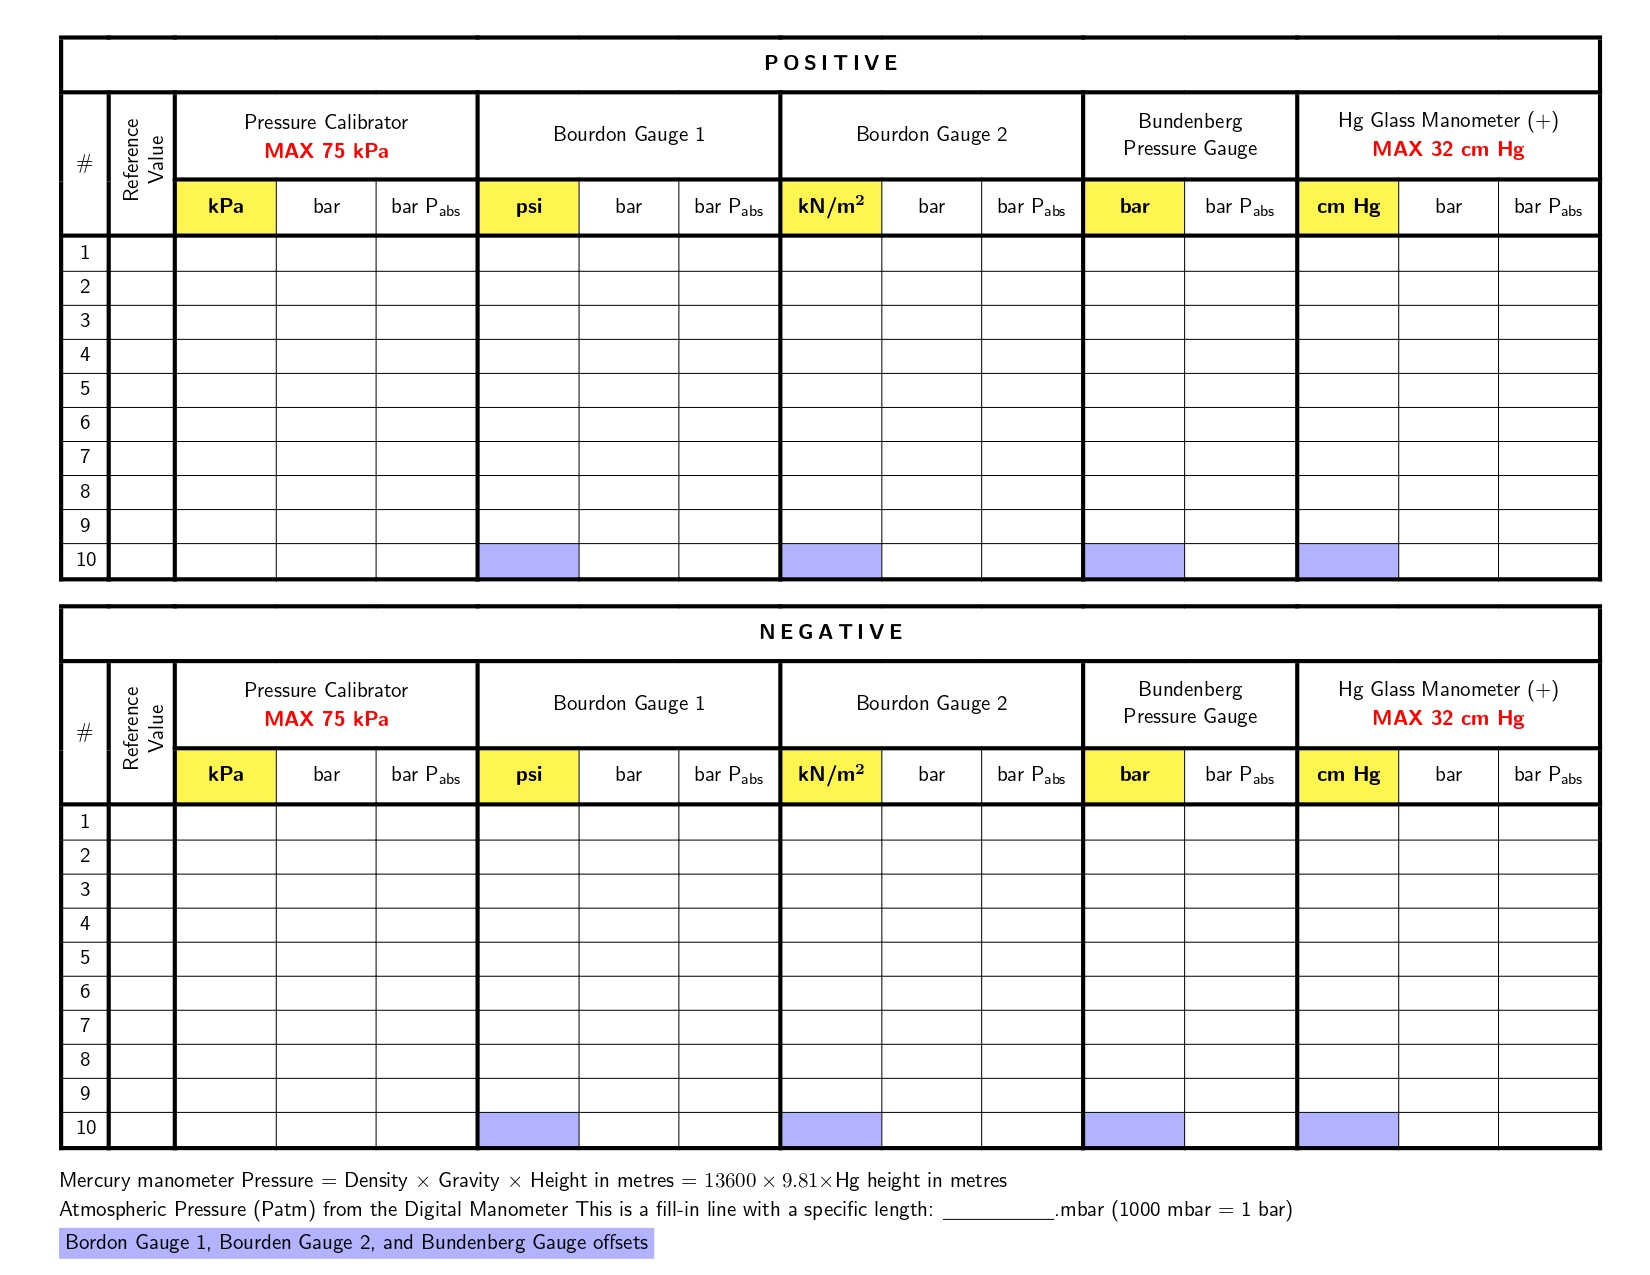
\includegraphics[width=1\textwidth,cfbox=gray!15 1pt]{images/tableland-1_page-0001.jpg} 
			\caption{Form for recording pressure measurements} 
			\label{fig:pressurestable} 
	\end{figure}
	\underline{The experiment \textbf{summary} is as follows:}\\[1em]
	The instructor provided us with a comprehensive demonstration on how to operate the pressure calibrator, guiding us through the process of setting up the equipment and interpreting the corresponding gauge readings.\\[1em]
	Prior to starting the experiment, we were given essential safety instructions, including precautions to prevent compromising our data and ensuring the safety of everyone involved.\\[1em]
	As the experiment progressed, we worked as a team to carefully apply the required pressures, analyzing the gauge readings and reaching a consensus on the correct values, which were then recorded in the designated pressure measurement table (Figure \ref{fig:pressurestable}).\\[1em]
	A detailed breakdown of the \textbf{exact steps} we followed is as follows:
\newpage
\newgeometry{left=0.8in,right=0.8in,top=1.3in,bottom=0.6in}
\begin{minipage}{0.5\textwidth}	
	\subsection{Operating Procedure}
	\begin{enumerate}[left=0in,itemsep=2mm]
	    \item The instructor inspected the test rig’s pneumatic connections to ensure they were secure.  
		\item The instrument’s vent valve was opened as part of the setup process.  
		\item Given the choice between vacuum (\textsf{\textcolor{blue}{-}}) and excess (\textsf{\textcolor{red}{+}}) pressure, we initially set the selector on the front of the DPI-603 ($\pm$VE in Figure \ref{fig:DPI-603}) to positive pressure. This setting allowed us to apply the necessary excess pressure for the procedure.  
		\item The unit was powered on by pressing the power button.  
		\item Using the pressure units button, we cycled through the available options (in Hg, bar, etc.) and selected kPa.  
	\end{enumerate}
\end{minipage}\hfill
\begin{minipage}{0.45\textwidth}
	\begin{figure}[H] 
		\centering 		
		\hspace*{-2em}
		\begin{tikzpicture}[scale=0.45,transform shape]
			\node[anchor=center] (image) at (0,0) {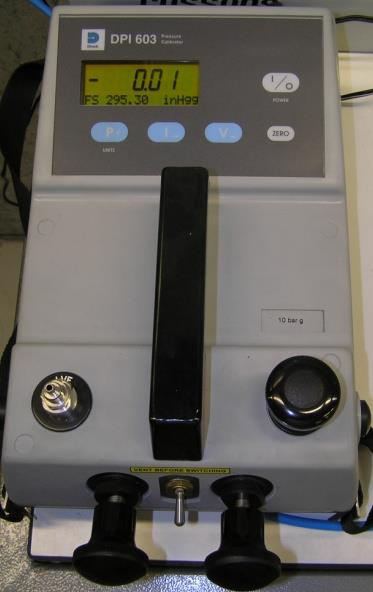
\includegraphics[width=1\textwidth]{extracted_images/image_8_1.png}};
     \draw[{Latex[length=3mm,width=3mm]}-,line width=0.5mm] (3.2, -2.2) -- (5, -3) node[above=1mm,right] {\Huge Vent Valve}; 
		     
		    \draw[{Latex[length=3mm,width=3mm]}-,line width=0.5mm] (-2, 3.4) -- (-5, 3) node[left=14mm,below=-10mm] {\Huge \wm{1}{Pressure\\ Units}}; 
		
		\draw[{Latex[length=3mm,width=3mm]}-,line width=0.5mm] (-0.15, -5) -- (-0.15, -8) node[below=1mm] {\Huge $\pm \text{VE}$}; 
		
		\draw[{Latex[length=3mm,width=3mm]}-,line width=0.5mm] (1.35, -6.3) -- (3, -8) node[below=6.5mm,right] {\Huge\text{Hand Pump}}; 
		
		\draw[{Latex[length=3mm,width=3mm]}-,line width=0.5mm] (1.35-3, -6.3) -- (-3, -8) node[below=5.9mm,left] {\Huge\text{Volume Control}}; 
		
		\draw[{Latex[length=3mm,width=3mm]}-,line width=0.5mm] (-1.5, 5) -- (-3.5, 7.4) node[above=5.9mm,left=-1cm] {\Huge\text{Main Display}}; 
		
		\draw[{Latex[length=3mm,width=3mm]}-,line width=0.5mm,draw=black] (2.5, 5) -- (4.3, 7.4) node[above=5.9mm,right=-1cm] {\Huge\text{Power}}; 
		
		\end{tikzpicture}
		\caption{DPI-603 Portable Pressure Calibrator} 
		\label{fig:DPI-603} 
	\end{figure}
\end{minipage}\\
\begin{enumerate}
\item[6.] The vent valve was closed and used to zero the instrument. It was concluded that this procedure should be carried out by the instructor due to the vent valve’s sensitivity.  
\end{enumerate}
\noindent
Here Steps 1–6 primarily cover the setup phase and were mainly carried out by the instructor. It was now our role to conduct the rest of the experiment, which proceeded as follows:

\begin{enumerate}
\item[7.] We used the hand pump to pressurize the system to the required value. To achieve precise control, we vented air using the vent valve and adjusted the pressure by pumping air as needed.
\item[8.] Once the required incremental was observed on the pressure calibrator, we then observe and recorded the readings seen on the following gauges:
\end{enumerate}

	\begin{minipage}{0.45\textwidth}
			\hspace{0.9em}\begin{minipage}{1\textwidth}\centering
			\begin{minipage}{0.45\textwidth}\centering
				
\includegraphics[width=1.2\textwidth]{images/Image(1).jpg}\\[0.5em]
				\rotatebox[origin=c]{0}{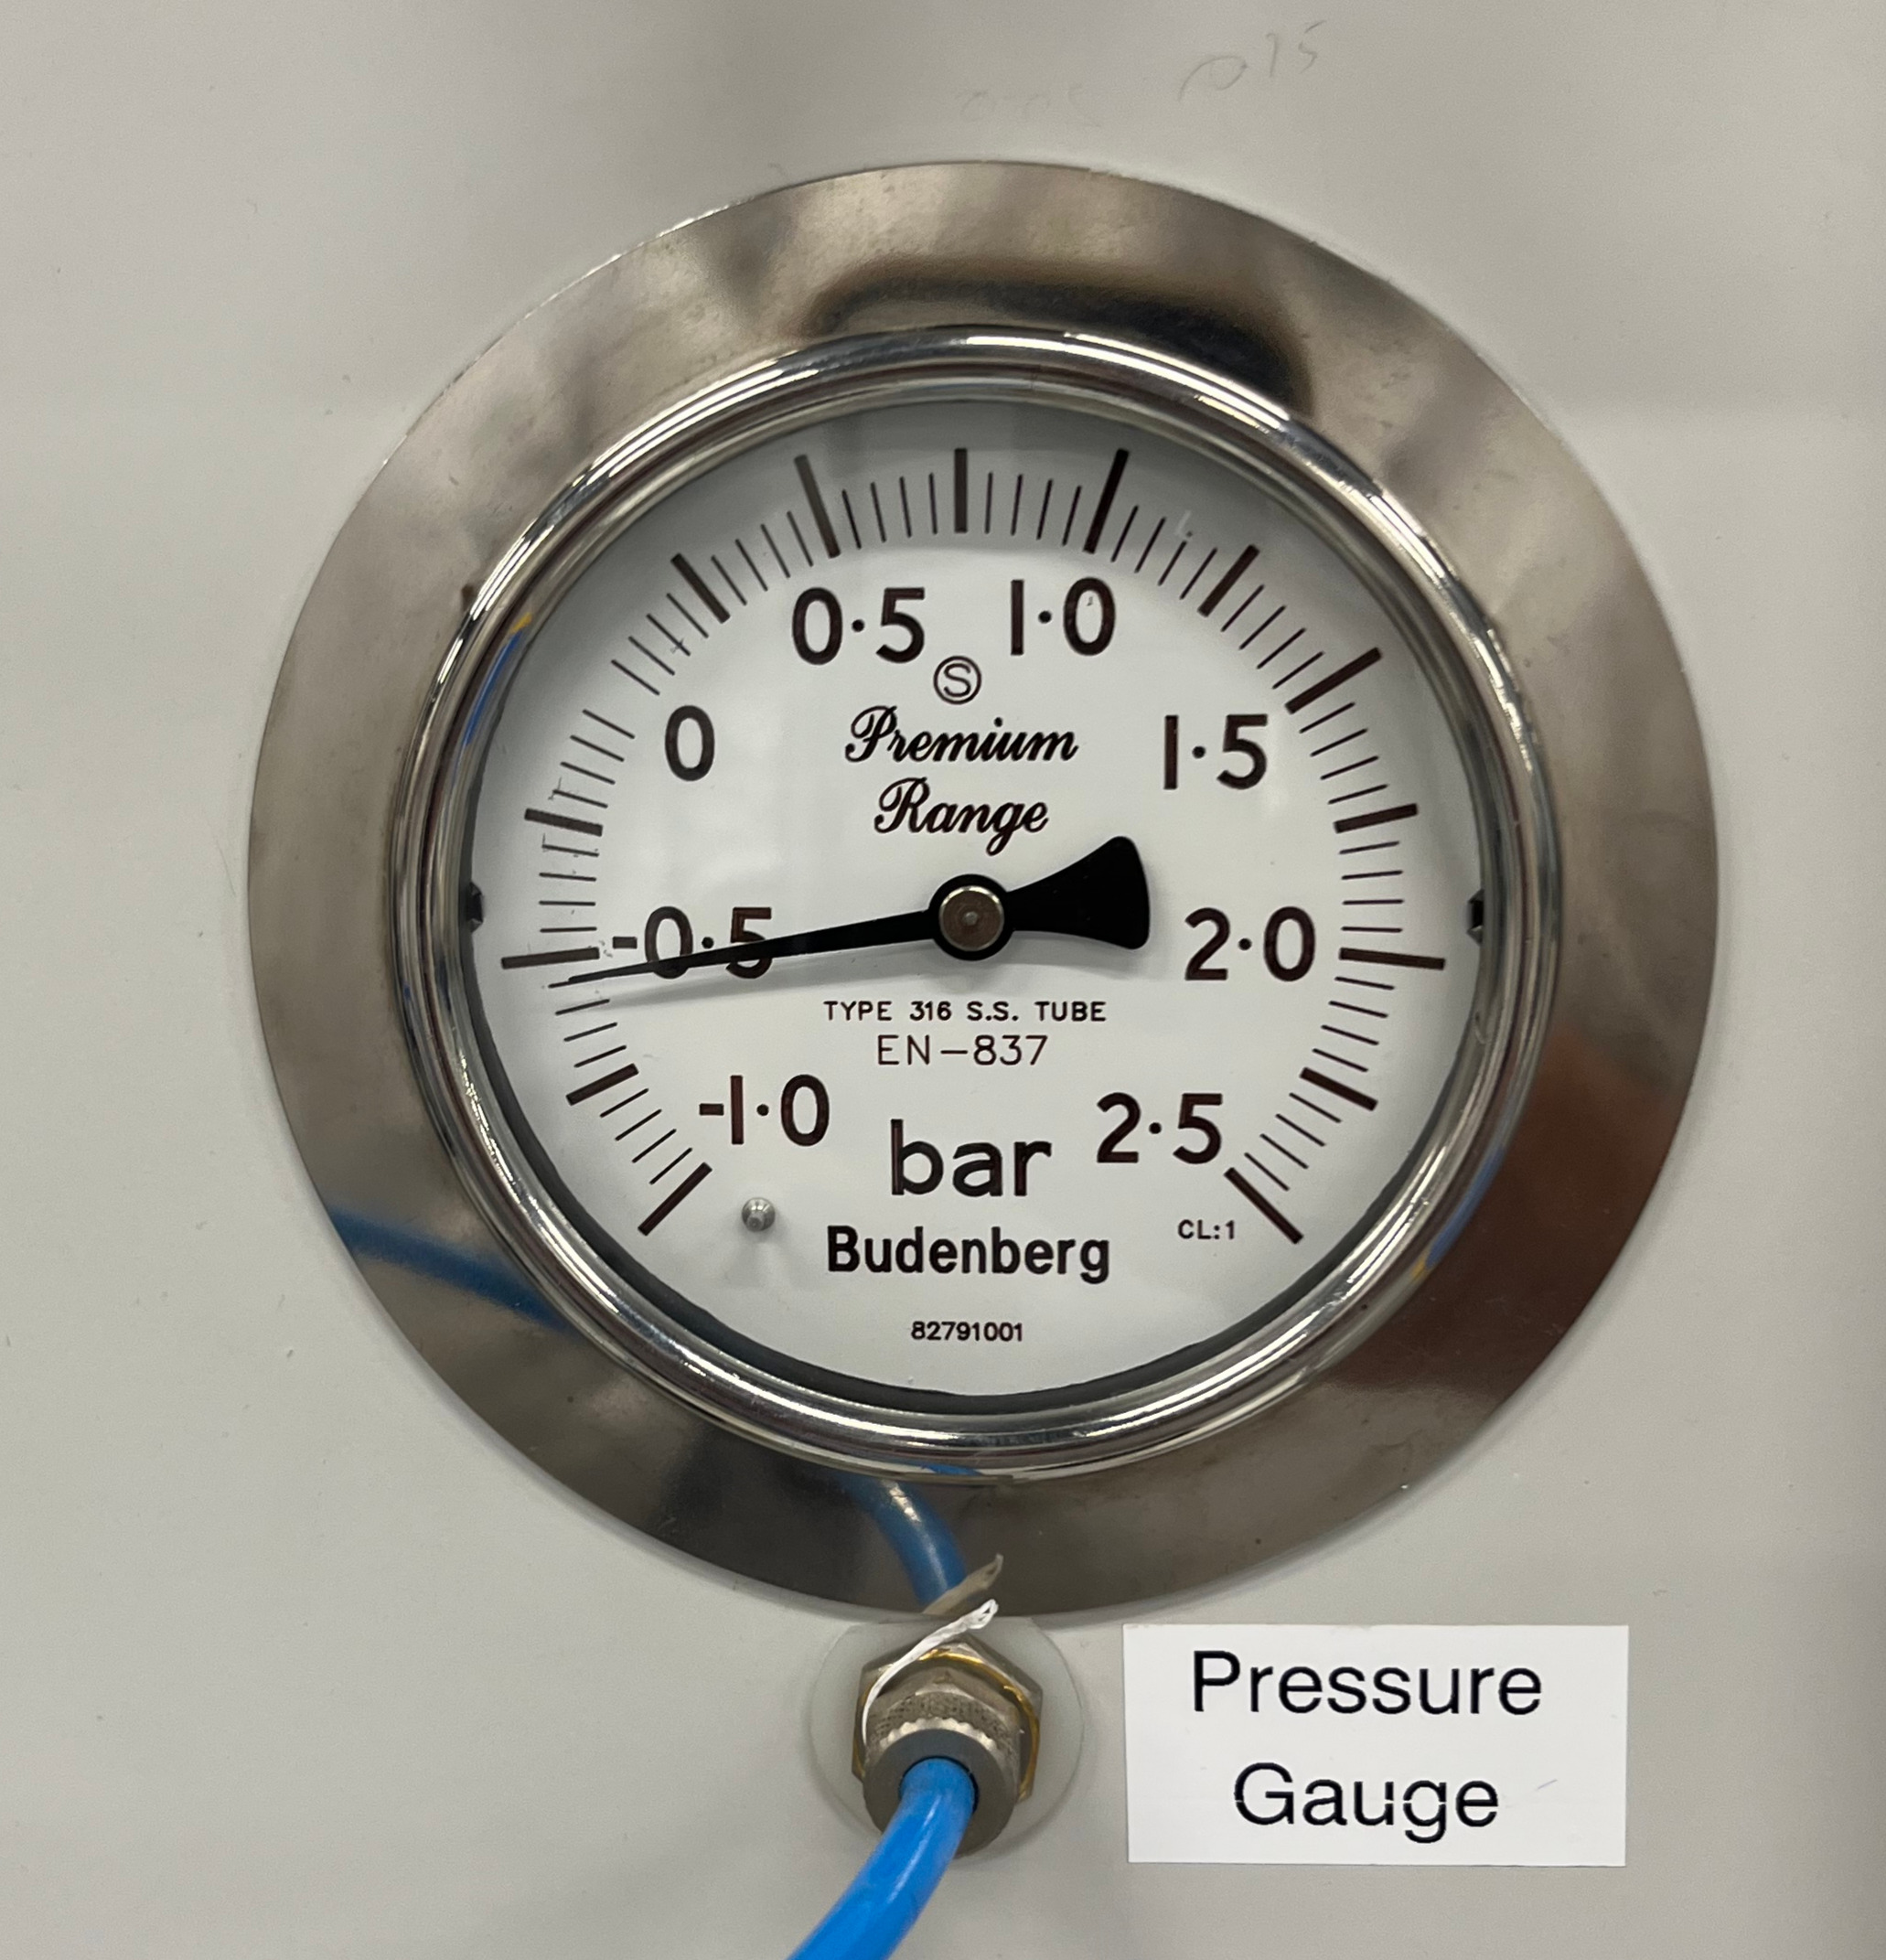
\includegraphics[width=1.2\textwidth]{images/Image(6).jpg}}
			\end{minipage}\hspace{0.5em}
			\begin{minipage}{0.4\textwidth}\centering
				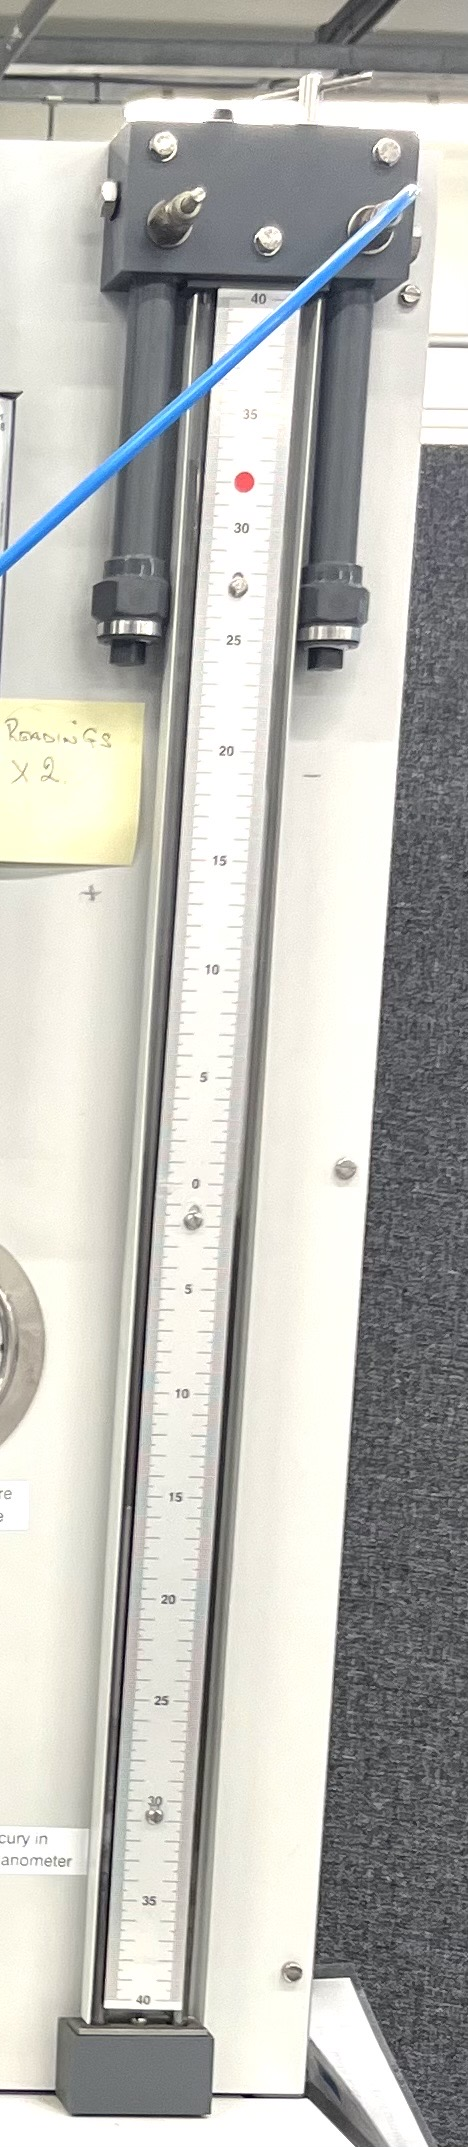
\includegraphics[width=0.55\textwidth]{images/Image(2).jpg}
			\end{minipage}
			\end{minipage}
			
			\centering
			\captionof{figure}{Gauges \& Manometer}\small Refer to Figure \ref{fig:pressure_measurement_bench} for illustrations labels.
	\end{minipage}
	\begin{minipage}{0.51\textwidth}\vspace{-2em}\raggedright
		\begin{enumerate}[left=0in]
			\item[9.]  By reaching on a agreement as a team over what is being read on the instruments for this related pressure value on the calibrator, we recorded them in the designated pressure measurement table (Figure \ref{fig:pressurestable}). 
			\item[10.] This procedure (Steps 7-9) is repeated, beginning with an \textbf{initial reading of 0 kPa} and continuing until the tenth increment, with each increment approximately $+5$ kPa.\\[-8pt]$$0,5,10, \ldots, 50$$\\[-6pt]
			\item[11.] Once we're done, we go back and repeat steps 6–10, except this time we do for the vacuum ($-5$kPa).
		\end{enumerate}\noindent
		This concludes everything that was done in the lab so that we may draw conclusions from the information in the tables.
	\end{minipage}
	
	\newpage\restoregeometry
	\section{Theory}
	
	\subsection{Pressure}
	
	When we talk about pressure, the first thing that comes to mind is its physical definition. It refers to the effect or various types of deflection when a force is applied to a surface.\vspace{-0.5em}
	\begin{center}
	\begin{minipage}{0.45\textwidth}
		\centering
		\begin{equation}
			P = \frac{F}{A}
			\label{eq:pressure}
		\end{equation}
		\hspace*{2em}\wm{0.9}{
		\begin{itemize}[itemsep=-1mm]
			\item \( P \) = Pressure (Pa, Pascal)
			\item \( F \) = Force applied (N, Newton)
			\item \( A \) = Surface area (m\(^2\))
		\end{itemize}
		}\\[1em]\raggedright
		"Pressure is the force per unit area exerted normal to the surface."
	\end{minipage}
	\hfil
	\begin{minipage}{0.45\textwidth}
		\centering
		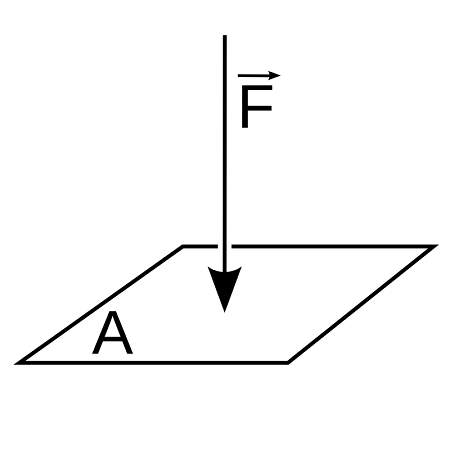
\includegraphics[width=0.6\textwidth]{images/pressure_force2652641600190961771.png}\vspace{-1.6em}
		\captionof{figure}{Illustration of pressure application}
		\label{fig:pressure}
	\end{minipage}\end{center}
	The type of deflection caused by pressure depends on its magnitude and the duration of application. Pressure has numerous examples and applications, such as vehicle tires and press machines.\\[1em]
	The most effective way to estimate applied pressure is by measuring its effects, for example, by observing changes in the dimensions of an elastic object or the height of a liquid column, as shown in the following image.
	\begin{figure}[H]
		\centering
		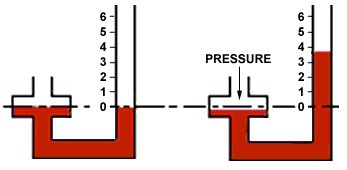
\includegraphics[width=0.5\textwidth]{images/Piezometer.jpg}
		\caption{Pressure measurement using a liquid column}
		\label{fig:piezometer}
	\end{figure}
	\noindent
	Pressure is categorized into two main groups: \textbf{gauge pressure} and \textbf{absolute pressure}, explained in the following diagram.
	\subsection{Absolute Pressure}
	Absolute pressure, or absolute zero pressure, is the lowest possible pressure measurable. Consequently, all measured pressures are positive in comparison to this reference point. Achieving absolute zero pressure is practically impossible unless calculated or represented through an extremely accurate curve.
	\subsection{Gauge Pressure}
	Gauge pressure, also known as relative pressure, is measured relative to local atmospheric pressure. Since we live under constant atmospheric pressure, it is often convenient to measure the difference between actual pressure and atmospheric pressure, which is referred to as gauge pressure. This measurement is commonly used in industrial applications.
	
	\newpage
	\noindent It is important to note that:\\[-5pt]
	\begin{itemize}
		\item Any pressure between local atmospheric pressure and absolute zero pressure is called \textbf{vacuum pressure}.
		\item Any pressure higher than local atmospheric pressure is considered \textbf{positive pressure}.
	\end{itemize}
	\vspace{0.7em}\noindent
	The relationship between absolute and gauge pressure is given by:\\[0.5em]
	\begin{equation}
		P_{\text{absolute}} = P_{\text{atmosphere}} + P_{\text{gauge}}
		\label{eq:absolute}
	\end{equation}\\
	\vspace{0.5em}
	The following diagram illustrates the definitions of pressure more clearly.	
	\begin{figure}[H]
		\centering
		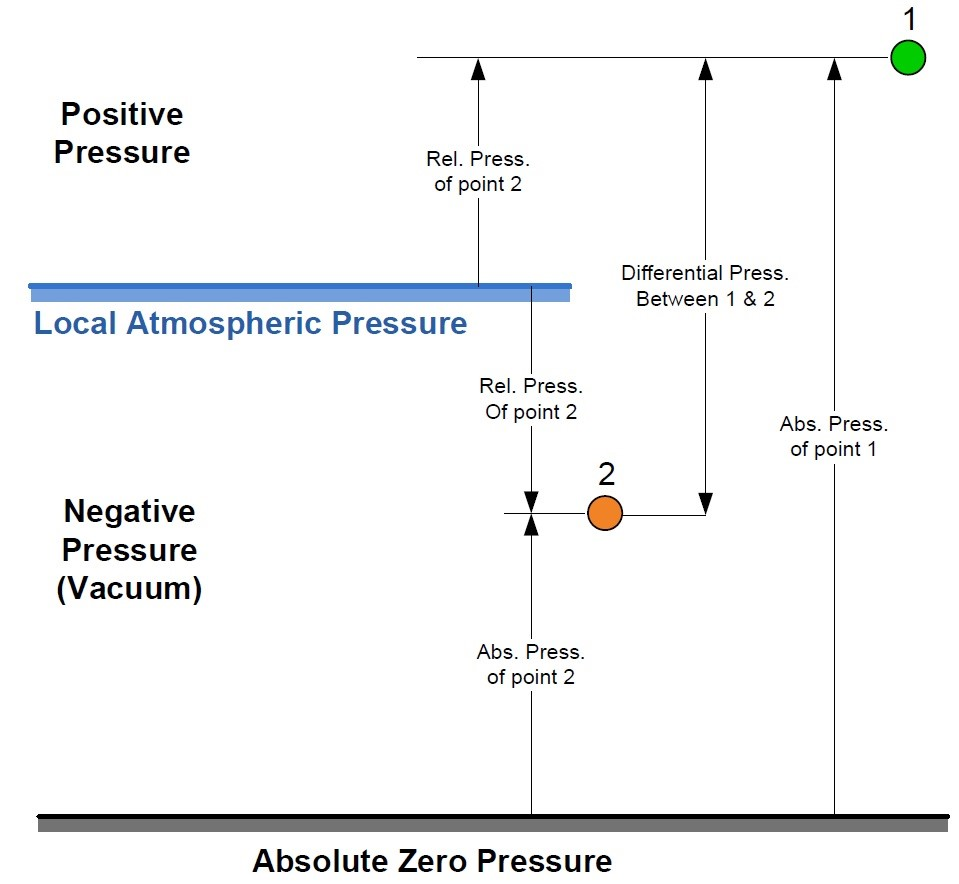
\includegraphics[width=0.95\textwidth]{images/Pressure Diagram.jpg}
		\caption{Pressure categories and their relationships}
		\label{fig:pressure_diagram}
	\end{figure}


	\newpage
	\subsection{How the instruments work}
	
	\newpage
	
	\subsection{Pressure Units}\label{Pressure Units}
The SI unit for pressure is the \textbf{Pascal (Pa)}, which is equivalent to \textbf{N/m\textsuperscript{2}} (Newton per square meter). Commonly used pressure units include \textbf{bar}, \textbf{psi} (pound per square inch), and \textbf{atm} (atmosphere). Below is a table of standard pressure units and their conversion factors:

\begin{table}[ht]
	\centering
	\begin{tabular}{lcccccc}
		\toprule
		\textbf{Unit} & \textbf{Pa} & \textbf{bar} & \textbf{psi} & \textbf{atm} & \textbf{cm Hg} \\
		\midrule
		Pa            & 1           & $1 \times 10^{-5}$ & $1.450 \times 10^{-4}$ & $9.869 \times 10^{-6}$ & $0.00750062$ \\
		bar           & $1 \times 10^{5}$ & 1            & 14.5038      & 0.986923     & 75.0062 \\
		psi           & 6894.76     & 0.0689476    & 1            & 0.068046     & 51.7149 \\
		atm           & 101325      & 1.01325      & 14.6959      & 1            & 76.0032 \\ 
		cm Hg         & 1333.22     & 0.013332     & 0.19337      & 0.013158     & 1 \\
		\bottomrule
	\end{tabular}
	\caption{Standard Pressure Unit Conversions}
	\label{tab:pressure_conversions}
\end{table}
\vspace{-2em}
\subsubsection{Pascal (Pa)}
The Pascal (Pa) is the SI unit of pressure, named after the French mathematician and physicist Blaise Pascal. It is defined as one Newton per square meter (\si{\newton\per\square\meter}). As a relatively small unit, the Pascal is commonly used in scientific fields such as laboratory research or atmospheric studies.
\subsubsection{Atmosphere (atm)}
The atmosphere (atm) is a unit of pressure defined as the average atmospheric pressure at sea level on Earth. Were \[1\,\text{atm}\approx101\, 325\,\text{Pa}\]
The atmosphere is commonly used in chemistry and physics to describe gas pressures, especially in contexts like gas laws (e.g., Boyle's Law and Charles's Law), as well as in scuba diving to describe underwater pressures. It is used for convenience, providing a standardized unit for atmospheric pressure in various scientific and engineering applications.
\subsubsection{Bar (bar)}
The bar is a metric unit of pressure, though it is not part of the International System of Units (SI). It is defined as \[1\,\text{bar}=100\, 000\,\text{Pa}\] 
This exact by definition. However, the relationship between bar and atm involves a small fractional difference due to the empirical value of standard atmospheric pressure, it is very close, specifically $$1\,\text{bar}\approx0.986923\,\text{atm}$$ Which is just 1.3077\% off. The bar is commonly used in meteorology, engineering, and industrial applications, as it provides a convenient scale for measuring pressures near atmospheric pressure.
\subsubsection{Pound per Square Inch (psi)}
The pound per square inch (psi) is a unit of pressure primarily used in the United States and other countries that follow the Imperial system. It is defined as the pressure exerted by one pound-force applied to an area of one square inch. PSI is widely used in automotive, mechanical engineering, and hydraulic systems, such as measuring tire pressure.\\[1em]
The conversion factor between psi and Pascal is given as:
\[1 \, \text{psi} = 6894.76 \, \text{Pa}.\]
This conversion is derived from the definition of the pound-force (lbf) and the inch.\\
One \textbf{pound-force (lbf)} is defined as the force required to accelerate a mass of one pound under the influence of gravity. In the metric system, 1 pound-force is approximately equivalent to 4.44822 Newtons (N). This is based on the following formulation:
\[1\,\text{lbf}=1\,\text{lb}\times g\]
\[1 \, \text{lbf} = 0.453592 \, \text{kg} \times 9.80665 \, \text{m/s}^2 = 4.44822 \, \text{N}.\]
The force of one pound-force is applied over an area of one square inch. One square inch is defined as:
\[1 \, \text{inch}^2 = 0.00064516 \, \text{m}^2.\]
Thus, the conversion from psi to Pascal is calculated by dividing the force in Newtons by the area in square meters:
\[1 \, \text{psi} = \frac{4.44822 \, \text{N}}{0.00064516 \, \text{m}^2} \approx 6894.76 \, \text{Pa}.\]
This precise conversion reflects the accurate definitions of the pound-force and the inch, with the result ensuring consistent and reliable unit conversion between the Imperial and SI systems.



	
	
	\newpage	
	\section{Data, Calculations and Results}
	In this section, we will present the calculations and results derived from the dataset collected during the experiment, as detailed in the \textbf{Method \& Experimental Procedures} section \ref{Method_Experimental_Procedures}. The primary objective is to analyze the data, identify trends, and generate additional information that will help us draw meaningful conclusions. To start, I will first describe the baseline data, which was recorded in the table provided for the lab (Figure \ref{fig:pressurestable}).
	
	\tikzexternaldisable

	
	\subsection{Pressure Readings}
	\begin{center}
	\begin{minipage}{0.23\textwidth}
		\begin{tcolorbox}[title={\color{black}\normalsize \textbf{Pressure Calibrator}}, colback=SkyBlue!6!white, 
			colframe=SteelBlue!10!white, boxrule=0.5mm, width=\textwidth]
		\hspace*{-0.82em}
		\begin{minipage}{1.2\textwidth}\centering
		\textbf{\textsf{kPa}}\\[8pt]
		\begin{tblr}{
					colspec={X[1cm]X[1cm]},
					hlines,vlines,
					cells={valign=m,halign=c,bg=white},
					rows={ht=1\baselineskip},
					row{1}={ht=1\baselineskip,font=\bfseries},
				}
				\Large\textsf{\textcolor{red}{+}}&\wm{0.2}{\vspace{0.1cm}\Large\textsf{\textcolor{blue}{-}}}\\\hline
				0  & 0  \\
				5.7  & -5.6  \\
				10.4 & -12.1 \\
				16.0 & -18.0 \\
				21.1 & -21.8 \\
				27.7 & -25.4 \\
				34.2 & -29.3 \\
				40.0 & -33.6 \\
				46.1 & -37.6 \\
				52.2 & -41.7 \\
			\end{tblr}
			\captionof{table}{Pressure Calibrator}
		\end{minipage}
		\end{tcolorbox}
	\end{minipage}
	\begin{minipage}{0.75\textwidth}
	\begin{tcolorbox}[
		title={\color{black}\normalsize \textbf{Pressure measuring instruments}},
		colback=MetallicSunburst!6!white, 
		colframe=ChineseGold!10!white, 
		boxrule=0.5mm, 
		width=1\textwidth
		]
		\begin{minipage}{1.03\textwidth}
			\hspace*{-1em}
			\centering	
			\begin{minipage}{0.225\textwidth}
			\centering
			\textbf{\textsf{psi}}\\[8pt]
			\begin{tblr}{
					colspec={X[1cm]X[1cm]},
					hlines,vlines,
					cells={valign=m,halign=c,bg=white},
					rows={ht=1\baselineskip},
					row{1}={ht=1\baselineskip,font=\bfseries},
				}
				\Large\textsf{\textcolor{red}{+}}&\wm{0.2}{\vspace{0.1cm}\Large\textsf{\textcolor{blue}{-}}}\\\hline
				1.0  & 1.2  \\
				2.0  & 0.4  \\
				2.6  & -0.5  \\
				3.4  & -2.0  \\
				4.1  & -2.8  \\
				5.0  & -4.0  \\
				6.0  & -6.0  \\
				6.8  & -7.1  \\
				7.6  & -8.3  \\
				8.5  & -9.5  \\
			\end{tblr}
			\captionof{table}{Bourdon Gauge 1}
		\end{minipage}
			\hfil
			\begin{minipage}{0.225\textwidth}
			\centering
			\textbf{\textsf{kN/m$\bm{^2}$}}\\[8pt]
			\begin{tblr}{
					colspec={X[1cm]X[1cm]},
					hlines,vlines,
					cells={valign=m,halign=c,bg=white},
					rows={ht=1\baselineskip},
					row{1}={ht=1\baselineskip,font=\bfseries},
				}
				\Large\textsf{\textcolor{red}{+}}&\wm{0.2}{\vspace{0.1cm}\Large\textsf{\textcolor{blue}{-}}}\\\hline
				1.0  & 2.5  \\
				8.0  & -1.0  \\
				14.0 & -9.0  \\
				20.0 & -15.0 \\
				25.0 & -20.0 \\
				30.0 & -23.0 \\
				39.0 & -27.0 \\
				45.0 & -32.0 \\
				50.0 & -36.0 \\
				57.0 & -40.0 \\
			\end{tblr}
			\captionof{table}{Bourdon Gauge 2}
		\end{minipage}
			\hfil
			\begin{minipage}{0.225\textwidth}
			\centering
			\textbf{\textsf{bar}}\\[8pt]
			\begin{tblr}{
					colspec={X[1cm]X[1cm]},
					hlines,vlines,
					cells={valign=m,halign=c,bg=white},
					rows={ht=1\baselineskip},
					row{1}={ht=1\baselineskip,font=\bfseries},
				}
				\Large\textsf{\textcolor{red}{+}}&\wm{0.2}{\vspace{0.1cm}\Large\textsf{\textcolor{blue}{-}}}\\\hline
				-0.05 & -0.05  \\
				0.00  & -0.10  \\
				0.04  & -0.16  \\
				0.10  & -0.24  \\
				0.15  & -0.27  \\
				0.22  & -0.30  \\
				0.29  & -0.35  \\
				0.35  & -0.40  \\
				0.40  & -0.44  \\
				0.47  & -0.49  \\
			\end{tblr}
			\captionof{table}{Budenberg Pressure Gauge}
		\end{minipage}
			\hfil
			\begin{minipage}{0.225\textwidth}
			\centering
			\textbf{\textsf{cm Hg}}\\[8pt]
			\begin{tblr}{
					colspec={X[1cm]X[1cm]},
					hlines,vlines,
					cells={valign=m,halign=c,bg=white},
					rows={ht=1\baselineskip},
					row{1}={ht=1\baselineskip,font=\bfseries},
				}
				\Large\textsf{\textcolor{red}{+}}&\wm{0.2}{\vspace{0.1cm}\Large\textsf{\textcolor{blue}{-}}}\\\hline
				0.4  & 0.4  \\
				3.5  & -0.7  \\
				5.3  & -3.7  \\
				7.4  & -5.4  \\
				9.4  & -6.8  \\
				11.6 & -8.2  \\
				14.2 & -9.6  \\
				16.4 & -11.3 \\
				18.7 & -12.8 \\
				21.0 & -14.4 \\
			\end{tblr}
			\captionof{table}{Hg Glass Manometer}
			\end{minipage}
		\end{minipage}		
		\end{tcolorbox}		
	\end{minipage}
	\end{center}
	As instructed, we first \textbf{zero out the data} by adjusting all values relative to the first element. This means that we subtract the first element from every value in the list. This ensures that the first element becomes zero, and the rest of the data maintains its relative differences. The specific reasonsing and justification for this is noted later.\\[1em] 
	The results are as follows:
	  
	  \newgeometry{left=0.8in,right=0.8in,top=1in,bottom=0.6in}
	  
\begin{center}
	\begin{minipage}{0.23\textwidth}
		\begin{tcolorbox}[title={\color{black}\normalsize \textbf{Pressure Calibrator}}, colback=SkyBlue!6!white, 
			colframe=SteelBlue!20!white, boxrule=0.5mm, width=\textwidth]
			\hspace*{-0.82em}
			\begin{minipage}{1.2\textwidth}\centering
				\textbf{\textsf{kPa}}\\[8pt]
				\begin{tblr}{
						colspec={X[1cm]X[1cm]},
						hlines,vlines,
						cells={valign=m,halign=c,bg=white},
						rows={ht=1\baselineskip},
						row{1}={ht=1\baselineskip,font=\bfseries},
					}
					\Large\textsf{\textcolor{red}{+}}&\wm{0.2}{\vspace{0.1cm}\Large\textsf{\textcolor{blue}{-}}}\\\hline
					0  & 0  \\
					5.7  & -5.6  \\
					10.4 & -12.1 \\
					16.0 & -18.0 \\
					21.1 & -21.8 \\
					27.7 & -25.4 \\
					34.2 & -29.3 \\
					40.0 & -33.6 \\
					46.1 & -37.6 \\
					52.2 & -41.7 \\
				\end{tblr}
				\captionof{table}{Pressure Calibrator (Zeroed)}
			\end{minipage}
		\end{tcolorbox}
	\end{minipage}
	\begin{minipage}{0.75\textwidth}
		\begin{tcolorbox}[
			title={\color{black}\normalsize \textbf{Pressure measuring instruments}},
			colback=MetallicSunburst!6!white, 
			colframe=ChineseGold!20!white, 
			boxrule=0.5mm, 
			width=1\textwidth
			]
			\begin{minipage}{1.03\textwidth}
				\hspace*{-1.5em}
				\centering	
				\begin{minipage}{0.22\textwidth}
					\centering
					\textbf{\textsf{psi}}\\[8pt]
					\begin{tblr}{
							colspec={X[1cm]X[1cm]},
							hlines,vlines,
							cells={valign=m,halign=c,bg=white},
							rows={ht=1\baselineskip},
							row{1}={ht=1\baselineskip,font=\bfseries},
						}
						\Large\textsf{\textcolor{red}{+}}&\wm{0.2}{\vspace{0.1cm}\Large\textsf{\textcolor{blue}{-}}}\\\hline
						0  & 0  \\
						1.0  & -0.8  \\
						1.6  & -1.7  \\
						2.4  & -3.2  \\
						3.1  & -4.0  \\
						4.0  & -5.2  \\
						5.0  & -7.2  \\
						5.8  & -8.3  \\
						6.6  & -9.5  \\
						7.5  & -10.7 \\
					\end{tblr}
					\captionof{table}{Bourdon Gauge 1 (Zeroed)}
				\end{minipage}
				\hfil
				\begin{minipage}{0.22\textwidth}
					\centering
					\textbf{\textsf{kN/m$\bm{^2}$}}\\[8pt]
					\begin{tblr}{
							colspec={X[1cm]X[1cm]},
							hlines,vlines,
							cells={valign=m,halign=c,bg=white},
							rows={ht=1\baselineskip},
							row{1}={ht=1\baselineskip,font=\bfseries},
						}
						\Large\textsf{\textcolor{red}{+}}&\wm{0.2}{\vspace{0.1cm}\Large\textsf{\textcolor{blue}{-}}}\\\hline
						0  & 0  \\
						7.0  & -3.5  \\
						13.0 & -11.5 \\
						19.0 & -17.5 \\
						24.0 & -22.5 \\
						29.0 & -25.5 \\
						38.0 & -29.5 \\
						44.0 & -34.5 \\
						49.0 & -38.5 \\
						56.0 & -42.5 \\
					\end{tblr}
					\captionof{table}{Bourdon Gauge 2 (Zeroed)}
				\end{minipage}
				\hfil
				\begin{minipage}{0.24\textwidth}
					\centering
					\textbf{\textsf{bar}}\\[8pt]
					\begin{tblr}{
							colspec={X[1cm]X[1cm]},
							hlines,vlines,
							cells={valign=m,halign=c,bg=white},
							rows={ht=1\baselineskip},
							row{1}={ht=1\baselineskip,font=\bfseries},
						}
						\Large\textsf{\textcolor{red}{+}}&\wm{0.2}{\vspace{0.1cm}\Large\textsf{\textcolor{blue}{-}}}\\\hline
						0 & 0  \\
						0.05 & -0.05  \\
						0.09 & -0.11  \\
						0.15 & -0.19  \\
						0.20 & -0.22  \\
						0.27 & -0.25  \\
						0.34 & -0.30  \\
						0.40 & -0.35  \\
						0.45 & -0.39  \\
						0.52 & -0.44  \\
					\end{tblr}
					\captionof{table}{Budenberg (Zeroed)}
				\end{minipage}
				\hfil
				\begin{minipage}{0.22\textwidth}
					\centering
					\textbf{\textsf{cm Hg}}\\[8pt]
					\begin{tblr}{
							colspec={X[1cm]X[1cm]},
							hlines,vlines,
							cells={valign=m,halign=c,bg=white},
							rows={ht=1\baselineskip},
							row{1}={ht=1\baselineskip,font=\bfseries},
						}
						\Large\textsf{\textcolor{red}{+}}&\wm{0.2}{\vspace{0.1cm}\Large\textsf{\textcolor{blue}{-}}}\\\hline
						0  & 0  \\
						3.1  & -1.1  \\
						4.9  & -4.1  \\
						7.0  & -5.8  \\
						9.0  & -7.2  \\
						11.2 & -8.6  \\
						13.8 & -10.0 \\
						16.0 & -11.7 \\
						18.3 & -13.2 \\
						20.6 & -14.8 \\
					\end{tblr}
					\captionof{table}{Hg Glass (Zeroed)}
				\end{minipage}
			\end{minipage}		
		\end{tcolorbox}		
	\end{minipage}
\end{center}
Now, we need to perform some unit conversions to ensure consistency across all measurements.\\[8pt]
In the context of this study, as seen in the table in Figure \ref{fig:pressurestable}, we are provided with a row for calculating bar and bar \(\text{P}_\text{abs}\), which directly suggests that all the pressures should be expressed in bar for all comparisons. In my opinion, the choice of unit doesn't significantly affect the results, when coming to conclusions we aim to achieve. I will demonstrate later in that the results are the same when using different units.\\[8pt]
That aside, here i covert them all to \textbf{bar}, using the relevnt calcs outlined in subsection \ref{Pressure Units}.

	\begin{center}
	\hspace*{-0.5em}\begin{minipage}{0.46\textwidth}\centering		
		\hspace*{-1em}\begin{tikzpicture}
			\begin{scope}		
				\draw[thick,->] 
				(-1,3.3) 
				.. controls (-0.5,4) and (1.6,4) .. 
				(2.4,3.3)  
				node[above,midway] {$\times 0.01$};
			\end{scope}

		\end{tikzpicture}\\
		\hspace*{1em}
	\begin{minipage}{1\textwidth}
	\begin{minipage}{0.4\textwidth}\centering
		\textbf{\textsf{kPa}}\\[8pt]
		\begin{tblr}{
				colspec={X[1cm]X[1cm]},
				hlines,vlines,
				cells={valign=m,halign=c,bg=white},
				rows={ht=1\baselineskip},
				row{1}={ht=1\baselineskip,font=\bfseries},
			}
			\Large\textsf{\textcolor{red}{+}} &\Large\textsf{\textcolor{blue}{-}} \\ \hline
			0  & 0  \\
			5.7  & -5.6  \\
			10.4 & -12.1 \\
			16.0 & -18.0 \\
			21.1 & -21.8 \\
			27.7 & -25.4 \\
			34.2 & -29.3 \\
			40.0 & -33.6 \\
			46.1 & -37.6 \\
			52.2 & -41.7 \\
		\end{tblr}
	\end{minipage}
	\begin{minipage}{0.43\textwidth}\centering
		\textbf{\textsf{Bar}}\\[8pt]
		\begin{tblr}{
				colspec={X[1.2cm]X[1.2cm]},
				hlines,vlines,
				cells={valign=m,halign=c,bg=white},
				rows={ht=1\baselineskip},
				row{1}={ht=1\baselineskip,font=\bfseries},
			}
			\Large\textsf{\textcolor{red}{+}} &\Large\textsf{\textcolor{blue}{-}} \\ \hline
			0 & 0 \\
			0.06 & -0.06 \\
			0.10 & -0.12 \\
			0.16 & -0.18 \\
			0.21 & -0.22 \\
			0.28 & -0.25 \\
			0.34 & -0.29 \\
			0.40 & -0.34 \\
			0.46 & -0.38 \\
			0.52 & -0.42 \\
		\end{tblr}
	\end{minipage}
	\end{minipage}
	\end{minipage}\hfil\vrule\hfil
	\hspace*{-0.5em}\begin{minipage}{0.46\textwidth}\centering		\hspace*{-1em}\begin{tikzpicture}
				\draw[thick,->] 
				(-1,3.3) 
				.. controls (-0.5,4) and (1.6,4) .. 
				(2.4,3.3)  
				node[above,midway] {$\times 0.0689$};
			\end{tikzpicture}\\
			\hspace*{1em}
			\begin{minipage}{1\textwidth}
				\begin{minipage}{0.4\textwidth}\centering
						\textbf{\textsf{psi}}\\[6pt]
						\begin{tblr}{
								colspec={X[1cm]X[1cm]},
								hlines,vlines,
								cells={valign=m,halign=c,bg=white},
								rows={ht=1\baselineskip},
								row{1}={ht=1\baselineskip,font=\bfseries},
							}
							\Large\textsf{\textcolor{red}{+}} &\Large\textsf{\textcolor{blue}{-}} \\ \hline
							0  & 0  \\
							1.0  & -0.8  \\
							1.6  & -1.7  \\
							2.4  & -3.2  \\
							3.1  & -4.0  \\
							4.0  & -5.2  \\
							5.0  & -7.2  \\
							5.8  & -8.3  \\
							6.6  & -9.5  \\
							7.5  & -10.7 \\
						\end{tblr}
				\end{minipage}
				\begin{minipage}{0.43\textwidth}\centering
						\textbf{\textsf{Bar}}\\[8pt]
						\begin{tblr}{
								colspec={X[1.2cm]X[1.2cm]},
								hlines,vlines,
								cells={valign=m,halign=c,bg=white},
								rows={ht=1\baselineskip},
								row{1}={ht=1\baselineskip,font=\bfseries},
							}
							\Large\textsf{\textcolor{red}{+}} &\Large\textsf{\textcolor{blue}{-}} \\ \hline
							0 & 0 \\
							0.07 & -0.06 \\
							0.11 & -0.12 \\
							0.17 & -0.22 \\
							0.21 & -0.28 \\
							0.28 & -0.36 \\
							0.34 & -0.5 \\
							0.4 & -0.57 \\
							0.46 & -0.66 \\
							0.52 & -0.74 \\
						\end{tblr}
				\end{minipage}
			\end{minipage}
	\end{minipage}
	\end{center}

	\restoregeometry\newpage
	\begin{center}
		\begin{minipage}{0.46\textwidth}\centering
				\hspace*{-1em}\begin{tikzpicture}
					\draw[thick,->] 
					(-1,3.3) 
					.. controls (-0.5,4) and (1.6,4) .. 
					(2.4,3.3)  
					node[above,midway] {$\times 0.01$};
				\end{tikzpicture}\\
				\hspace*{1em}
				\begin{minipage}{1\textwidth}
					\begin{minipage}{0.4\textwidth}\centering
							\textbf{\textsf{kN/m$\bm{^2}$}}\\[8pt]
							\begin{tblr}{
									colspec={X[1cm]X[1cm]},
									hlines,vlines,
									cells={valign=m,halign=c,bg=white},
									rows={ht=1\baselineskip},
									row{1}={ht=1\baselineskip,font=\bfseries},
								}
								\Large\textsf{\textcolor{red}{+}} &\Large\textsf{\textcolor{blue}{-}} \\ \hline
								0.0  & 0.0  \\
								7.0  & -3.5  \\
								13.0 & -11.5 \\
								19.0 & -17.5 \\
								24.0 & -22.5 \\
								29.0 & -25.5 \\
								38.0 & -29.5 \\
								44.0 & -34.5 \\
								49.0 & -38.5 \\
								56.0 & -42.5 \\
							\end{tblr}
					\end{minipage}
					\begin{minipage}{0.43\textwidth}\centering
							\textbf{\textsf{Bar}}\\[8pt]
							\begin{tblr}{
									colspec={X[1.2cm]X[1.2cm]},
									hlines,vlines,
									cells={valign=m,halign=c,bg=white},
									rows={ht=1\baselineskip},
									row{1}={ht=1\baselineskip,font=\bfseries},
								}
								\Large\textsf{\textcolor{red}{+}} &\Large\textsf{\textcolor{blue}{-}} \\ \hline
							    0  &  0 \\
							    0.07  & -0.04  \\
							    0.13  & -0.12  \\
							    0.19  & -0.18  \\
							    0.24  & -0.23  \\
							    0.29  & -0.26  \\
							    0.38  & -0.30  \\
							    0.44  & -0.35  \\
							    0.49  & -0.39  \\
							    0.56  & -0.43  \\
							\end{tblr}
					\end{minipage}
				\end{minipage}
		\end{minipage}
		\hfil\vrule\hfil\begin{minipage}{0.46\textwidth}\centering
				\hspace*{-1em}\begin{tikzpicture}
					\draw[thick,->] 
					(-1,3.3) 
					.. controls (-0.5,4) and (1.6,4) .. 
					(2.4,3.3)  
					node[above,midway] {$\times 0.01333$};
				\end{tikzpicture}\\
				\hspace*{1em}
				\begin{minipage}{1\textwidth}
					\begin{minipage}{0.4\textwidth}\centering
							\textbf{\textsf{cm Hg}}\\[8pt]
							\begin{tblr}{
									colspec={X[1cm]X[1cm]},
									hlines,vlines,
									cells={valign=m,halign=c,bg=white},
									rows={ht=1\baselineskip},
									row{1}={ht=1\baselineskip,font=\bfseries},
								}
								\Large\textsf{\textcolor{red}{+}} &\Large\textsf{\textcolor{blue}{-}} \\ \hline
								0  & 0  \\
								3.1  & -1.1  \\
								4.9  & -4.1  \\
								7.0  & -5.8  \\
								9.0  & -7.2  \\
								11.2 & -8.6  \\
								13.8 & -10.0 \\
								16.0 & -11.7 \\
								18.3 & -13.2 \\
								20.6 & -14.8 \\
							\end{tblr}
					\end{minipage}
					\begin{minipage}{0.43\textwidth}\centering
							\textbf{\textsf{Bar}}\\[8pt]
							\begin{tblr}{
									colspec={X[1.2cm]X[1.2cm]},
									hlines,vlines,
									cells={valign=m,halign=c,bg=white},
									rows={ht=1\baselineskip},
									row{1}={ht=1\baselineskip,font=\bfseries},
								}
								\Large\textsf{\textcolor{red}{+}} &\Large\textsf{\textcolor{blue}{-}} \\ \hline
							0 & 0 \\
							0.04 & -0.01 \\
							0.07 & -0.05 \\
							0.09 & -0.08 \\
							0.12 & -0.10 \\
							0.15 & -0.11 \\
							0.18 & -0.13 \\
							0.21 & -0.16 \\
							0.24 & -0.18 \\
							0.27 & -0.20 \\
							\end{tblr}
					\end{minipage}
				\end{minipage}
		\end{minipage}
	\end{center}
	
	
	
	\begin{center}
		\begin{minipage}{0.23\textwidth}
			\begin{tcolorbox}[title={\color{black}\normalsize \textbf{Pressure Calibrator}}, colback=SkyBlue!6!white, 
				colframe=SteelBlue!30!white, boxrule=0.5mm, width=\textwidth]
				\hspace*{-0.82em}
				\begin{minipage}{1.2\textwidth}\centering
					\textbf{\textsf{Bar}}\\[8pt]
					\begin{tblr}{
							colspec={X[1cm]X[1cm]},
							hlines,vlines,
							cells={valign=m,halign=c,bg=white},
							rows={ht=1\baselineskip},
							row{1}={ht=1\baselineskip,font=\bfseries},
						}
						\Large\textsf{\textcolor{red}{+}}&\wm{0.2}{\vspace{0.1cm}\Large\textsf{\textcolor{blue}{-}}}\\\hline
						0  & 0  \\
						0.06  & -0.06  \\
						0.10  & -0.12  \\
						0.16  & -0.18  \\
						0.21  & -0.22  \\
						0.28  & -0.25  \\
						0.34  & -0.29  \\
						0.40  & -0.34  \\
						0.46  & -0.38  \\
						0.52  & -0.42  \\
					\end{tblr}
					\captionof{table}{Pressure Calibrator as bar}
				\end{minipage}
			\end{tcolorbox}
		\end{minipage}
		\begin{minipage}{0.75\textwidth}
			\begin{tcolorbox}[
				title={\color{black}\normalsize \textbf{Pressure measuring instruments}},
				colback=MetallicSunburst!6!white, 
				colframe=ChineseGold!30!white, 
				boxrule=0.5mm, 
				width=1\textwidth
				]
				\begin{minipage}{1.03\textwidth}
					\hspace*{-1.5em}
					\centering	
					\begin{minipage}{0.22\textwidth}
						\centering
						\textbf{\textsf{Bar}}\\[8pt]
						\begin{tblr}{
								colspec={X[1cm]X[1cm]},
								hlines,vlines,
								cells={valign=m,halign=c,bg=white},
								rows={ht=1\baselineskip},
								row{1}={ht=1\baselineskip,font=\bfseries},
							}
							\Large\textsf{\textcolor{red}{+}}&\wm{0.2}{\vspace{0.1cm}\Large\textsf{\textcolor{blue}{-}}}\\\hline
							0  & 0  \\
							0.07  & -0.06  \\
							0.11  & -0.12  \\
							0.17  & -0.22  \\
							0.21  & -0.28  \\
							0.28  & -0.36  \\
							0.34  & -0.50  \\
							0.4  & -0.57  \\
							0.46  & -0.66  \\
							0.52  & -0.74  \\
						\end{tblr}
						\captionof{table}{Bourdon Gauge 1 as bar}
					\end{minipage}
					\hfil
					\begin{minipage}{0.22\textwidth}
						\centering
						\textbf{\textsf{Bar}}\\[8pt]
						\begin{tblr}{
								colspec={X[1cm]X[1cm]},
								hlines,vlines,
								cells={valign=m,halign=c,bg=white},
								rows={ht=1\baselineskip},
								row{1}={ht=1\baselineskip,font=\bfseries},
							}
							\Large\textsf{\textcolor{red}{+}}&\wm{0.2}{\vspace{0.1cm}\Large\textsf{\textcolor{blue}{-}}}\\\hline
							0  & 0  \\
							0.07  & -0.04  \\
							0.13  & -0.12  \\
							0.19  & -0.18  \\
							0.24  & -0.23  \\
							0.29  & -0.26  \\
							0.38  & -0.30  \\
							0.44  & -0.35  \\
							0.49  & -0.39  \\
							0.56  & -0.43  \\
						\end{tblr}
						\captionof{table}{Bourdon Gauge 2 as bar}
					\end{minipage}
					\hfil
					\begin{minipage}{0.24\textwidth}
						\vspace{-1em}\centering
						\textbf{\textsf{Bar}}\\[8pt]
						\begin{tblr}{
								colspec={X[1cm]X[1cm]},
								hlines,vlines,
								cells={valign=m,halign=c,bg=white},
								rows={ht=1\baselineskip},
								row{1}={ht=1\baselineskip,font=\bfseries},
							}
							\Large\textsf{\textcolor{red}{+}}&\wm{0.2}{\vspace{0.1cm}\Large\textsf{\textcolor{blue}{-}}}\\\hline
							0 & 0  \\
							0.05 & -0.05  \\
							0.09 & -0.11  \\
							0.15 & -0.19  \\
							0.20 & -0.22  \\
							0.27 & -0.25  \\
							0.34 & -0.30  \\
							0.40 & -0.35  \\
							0.45 & -0.39  \\
							0.52 & -0.44  \\
						\end{tblr}
						\captionof{table}{Budenberg}
					\end{minipage}
					\hfil
					\begin{minipage}{0.22\textwidth}
						\centering
						\textbf{\textsf{Bar}}\\[8pt]
						\begin{tblr}{
								colspec={X[1cm]X[1cm]},
								hlines,vlines,
								cells={valign=m,halign=c,bg=white},
								rows={ht=1\baselineskip},
								row{1}={ht=1\baselineskip,font=\bfseries},
							}
							\Large\textsf{\textcolor{red}{+}}&\wm{0.2}{\vspace{0.1cm}\Large\textsf{\textcolor{blue}{-}}}\\\hline
							0  & 0  \\
							0.04  & -0.01  \\
							0.07  & -0.05  \\
							0.09  & -0.08  \\
							0.12  & -0.10  \\
							0.15  & -0.11  \\
							0.18  & -0.13  \\
							0.21  & -0.16  \\
							0.24  & -0.18  \\
							0.27  & -0.20  \\
						\end{tblr}
						\captionof{table}{Hg Glass as bar}
					\end{minipage}
				\end{minipage}		
			\end{tcolorbox}		
		\end{minipage}
	\end{center}
	
	\tikzexternalenable\newpage	  \newgeometry{left=0.8in,right=0.8in,top=0.9in,bottom=0.56in}
	
	\subsection{Borden Gauge 1 vs Calibrator}
	\newcommand{\datadir}{data/same_units}
	\newcommand{\instrumentfile}{Bourden_Gauge_bar.csv}
	\pgfplotstableread[col sep=comma]{\datadir/\instrumentfile}\instrumenttable
	\pgfplotstableread[col sep=comma]{\datadir/Pressure_Calibrator_bar.csv}\calibratortable
	\StrBefore{\instrumentfile}{_bar.csv}[\instrumentname]
	\StrSubstitute{\instrumentname}{_}{ }[\instrumentnameformatted]

	\hspace*{-3em}
	\begin{minipage}{1.2\textwidth}	
	\begin{minipage}[t]{0.3\textwidth}\centering\vspace{0pt}
	\begin{tikzpicture}[scale=0.8,transform shape]
		\begin{axis}[
			xlabel={\instrumentnameformatted\ (bar)},
			ylabel={Pressure Calibrator (bar)},
			axis lines=middle, 
			grid=both,
			legend pos=north west,
			xlabel style={
				at={(0.72,-0.15)}, 
			},
			ylabel style={
				at={(-0.16,0.5)},
				rotate=-90, 
			},
			xtick={0.1,0.2,0.3,0.4,0.5,0.6}, 
			ytick={0.1,0.2,0.3,0.4,0.5,0.6},
			xmin=0, xmax=0.6, 
			ymax=0.6, ymin=0,
			font=\small,
			tick label style={font=\tiny},
			label style={font=\footnotesize},
			legend style={font=\tiny},
			]
			\pgfplotsinvokeforeach{0,1,2,3,4,5,6,7,8,9} {
				\pgfplotstablegetelem{#1}{Positive}\of\instrumenttable
				\edef\xvalue{\pgfplotsretval}
				\pgfplotstablegetelem{#1}{Positive}\of\calibratortable
				\edef\yvalue{\pgfplotsretval}
				\addplot[only marks, mark=*, red] coordinates {(\xvalue, \yvalue)};
			};
			\addplot[
			domain=0:0.7, 
			samples=100,
			color=red,
			opacity=0.6,
			dashed,
			] {1.0224*x + -0.0074};
			\addplot[
			domain=0:0.6, 
			samples=100,
			color=black,
			opacity=0.3,
			] {x};
			\legend{Positive Data,Best Fit}
		\end{axis}
	\end{tikzpicture}
	\end{minipage}\hspace{1em}
	\begin{minipage}[t]{0.3\textwidth}\centering\vspace{0pt}
	\vspace*{-1em}
	\begin{tikzpicture}[scale=0.8,transform shape]
		\begin{axis}[
			xlabel={\instrumentnameformatted\ (bar)},
			ylabel={Pressure Calibrator (bar)},
			axis lines=middle, 
			grid=both,
			legend pos=north west,legend style={font=\tiny, yshift=-10pt},
			xlabel style={
				at={(0.71,1.025)}, 
			},
			ylabel style={
				at={(1.025,0.5)},
				rotate=-90, 
			},
			xtick={-0.7,-0.6,-0.5,-0.4,-0.3,-0.2,-0.1,0}, 
			ytick={-0.5,-0.4,-0.3,-0.2,-0.1,0},
			xmin=-0.77, xmax=0, 
			ymin=-0.52, ymax=0,
			axis line style={stealth-}, 
			font=\small,
			tick label style={font=\tiny},
			label style={font=\footnotesize},
			legend style={font=\tiny},
			]
			\pgfplotsinvokeforeach{0,1,2,3,4,5,6,7,8,9} {
				\pgfplotstablegetelem{#1}{Negative}\of\instrumenttable
				\edef\xvalue{\pgfplotsretval}
				\pgfplotstablegetelem{#1}{Negative}\of\calibratortable
				\edef\yvalue{\pgfplotsretval}
				\addplot[only marks, mark=*, blue] coordinates {(\xvalue, \yvalue)};
			};
			\addplot[
			domain=0:-0.75, 
			samples=100,
			color=blue,
			opacity=0.6,
			dashed,
			] {0.5241*x + -0.0423};
			\addplot[
			domain=0:-0.6, 
			samples=100,
			color=black,
			opacity=0.3,
			] {x};
			\legend{Negative Data,Best Fit}
		\end{axis}
	\end{tikzpicture}
	\end{minipage}\hspace{2em}\hspace{-1.7em}
	\begin{minipage}[t]{0.3\textwidth}\centering\vspace{0pt}
	\begin{tikzpicture}[scale=0.83,transform shape]
		\begin{axis}[
			xlabel={\instrumentnameformatted\ (bar)},
			ylabel={Pressure Calibrator (bar)},
			axis lines=middle, 
			grid=both,
			legend pos=north west,
			xlabel style={
				at={(0.7,-0.1)}, 
			},
			ylabel style={
				at={(1.02,0.5)},
				rotate=-90, 
			},
			xtick={-0.1,-0.2,-0.3,-0.4,-0.5,-0.6,-0.7,0.1,0.2,0.3,0.4,0.5,0.6,0.7,0.8}, 
			ytick={-0.1,-0.2,-0.3,-0.4,-0.5,-0.6,0.1,0.2,0.3,0.4,0.5,0.6},
			xmin=-0.8, xmax=0.7, 
			ymax=0.7, ymin=-0.5,
			font=\small,
			tick label style={font=\tiny},
			label style={font=\footnotesize},
			legend style={font=\tiny},
			]
			\pgfplotsinvokeforeach{0,1,2,3,4,5,6,7,8,9} {
				\pgfplotstablegetelem{#1}{Positive}\of\instrumenttable
				\edef\xvalue{\pgfplotsretval}
				\pgfplotstablegetelem{#1}{Positive}\of\calibratortable
				\edef\yvalue{\pgfplotsretval}
				\addplot[only marks, mark=*, red] coordinates {(\xvalue, \yvalue)};
			};
			\pgfplotsinvokeforeach{0,1,2,3,4,5,6,7,8,9} {
				\pgfplotstablegetelem{#1}{Negative}\of\instrumenttable
				\edef\xvalue{\pgfplotsretval}
				\pgfplotstablegetelem{#1}{Negative}\of\calibratortable
				\edef\yvalue{\pgfplotsretval}
				\addplot[only marks, mark=*, blue] coordinates {(\xvalue, \yvalue)};
			};
			\addplot[
			domain=-0.7:0.7, 
			samples=100,
			color=black,
			opacity=0.6,
			dashed,
			] {0.7554*x + 0.0496};
			\addplot[
			domain=-0.6:0.6, 
			samples=100,
			color=black,
			opacity=0.3,
			] {x};
			\legend{Positive Data, Negative Data, Combined Fit}
		\end{axis}
	\end{tikzpicture}	\end{minipage}
	\end{minipage}\vspace{-0.4em}
	\begin{center}
		\hspace*{-2em}
		\begin{minipage}{1.1\textwidth}
			\begin{minipage}{0.3\textwidth}	\centering
				Positive, best-fit equation: 
				\[y = 1.0224x + -0.0074\]
			\end{minipage}\hfill
			\begin{minipage}{0.3\textwidth}	\centering
				Negative, best-fit equation: 
				\[y = 0.5241x + -0.0423\]
			\end{minipage}\hfill
			\begin{minipage}{0.3\textwidth}	\centering
				Combined, best-fit equation: 
				\[y = 0.7554x + 0.0496\]
			\end{minipage}
		\end{minipage}
	\end{center}

	
	\subsection{Borden Gauge 2 vs Calibrator}
	
	\newcommand{\instrumentfiletwo}{Bourden_Gauge_2_bar.csv}
	\pgfplotstableread[col sep=comma]{\datadir/\instrumentfiletwo}\instrumenttabletwo
	
	\StrBefore{\instrumentfiletwo}{_bar.csv}[\instrumentnametwo]
	\StrSubstitute{\instrumentnametwo}{_}{ }[\instrumentnameformattedtwo]
	
	\hspace*{-3em}
	\begin{minipage}{1.2\textwidth}	
		\begin{minipage}[t]{0.3\textwidth}\centering\vspace{0pt}
			\begin{tikzpicture}[scale=0.8,transform shape]
				\begin{axis}[
					xlabel={\instrumentnameformattedtwo\ (bar)},
					ylabel={Pressure Calibrator (bar)},
					axis lines=middle, 
					grid=both,
					legend pos=north west,
					xlabel style={
						at={(0.72,-0.15)}, 
					},
					ylabel style={
						at={(-0.16,0.5)},
						rotate=-90, 
					},
					xtick={0.1,0.2,0.3,0.4,0.5,0.6}, 
					ytick={0.1,0.2,0.3,0.4,0.5,0.6},
					xmin=0, xmax=0.6, 
					ymax=0.6, ymin=0,
					font=\small,
					tick label style={font=\tiny},
					label style={font=\footnotesize},
					legend style={font=\tiny},
					]
					\pgfplotsinvokeforeach{0,1,2,3,4,5,6,7,8,9} {
						\pgfplotstablegetelem{#1}{Positive}\of\instrumenttabletwo
						\edef\xvalue{\pgfplotsretval}
						\pgfplotstablegetelem{#1}{Positive}\of\calibratortable
						\edef\yvalue{\pgfplotsretval}
						\addplot[only marks, mark=*, red] coordinates {(\xvalue, \yvalue)};
					};


					\addplot[
					domain=0:0.6, 
					samples=100,
					color=red,
					opacity=0.6,
					dashed,
					] {0.9462*x-0.0106};
					\addplot[
					domain=0:0.6, 
					samples=100,
					color=black,
					opacity=0.3,
					] {x};
					\legend{Positive Data,Best Fit}
				\end{axis}			
			\end{tikzpicture}
		\end{minipage}\hspace{1em}
		\begin{minipage}[t]{0.3\textwidth}\centering\vspace{0pt}
			\vspace*{-1em}
			\begin{tikzpicture}[scale=0.8,transform shape]
				\begin{axis}[
					xlabel={\instrumentnameformattedtwo\ (bar)},
					ylabel={Pressure Calibrator (bar)},
					axis lines=middle, 
					grid=both,
					legend pos=north west,legend style={font=\tiny, yshift=-10pt},
					xlabel style={
						at={(0.71,1.025)}, 
					},
					ylabel style={
						at={(1.025,0.5)},
						rotate=-90, 
					},
					xtick={-0.5,-0.4,-0.3,-0.2,-0.1}, 
					ytick={-0.5,-0.4,-0.3,-0.2,-0.1},
					xmin=-0.5, xmax=0, 
					ymin=-0.5, ymax=0,
					axis line style={stealth-}, 
					font=\small,
					tick label style={font=\tiny},
					label style={font=\footnotesize},
					legend style={font=\tiny},
					]
					\pgfplotsinvokeforeach{0,1,2,3,4,5,6,7,8,9} {
						\pgfplotstablegetelem{#1}{Negative}\of\instrumenttabletwo
						\edef\xvalue{\pgfplotsretval}
						\pgfplotstablegetelem{#1}{Negative}\of\calibratortable
						\edef\yvalue{\pgfplotsretval}
						\addplot[only marks, mark=*, blue] coordinates {(\xvalue, \yvalue)};
					};


					\addplot[
					domain=0:-0.5, 
					samples=100,
					color=blue,
					opacity=0.6,
					dashed,
					] {0.9509*x -0.0107};
					\addplot[
					domain=0:-0.5, 
					samples=100,
					color=black,
					opacity=0.3,
					] {x};
					\legend{Negative Data,Best Fit}
				\end{axis}
			\end{tikzpicture}
		\end{minipage}\hspace{2em}\hspace{-1.7em}
		\begin{minipage}[t]{0.3\textwidth}\centering\vspace{0pt}
			\begin{tikzpicture}[scale=0.83,transform shape]
				\begin{axis}[
					xlabel={\instrumentnameformattedtwo\ (bar)},
					ylabel={Pressure Calibrator (bar)},
					axis lines=middle, 
					grid=both,
					legend pos=north west,
					xlabel style={
						at={(0.7,-0.1)}, 
					},
					ylabel style={
						at={(1.02,0.5)},
						rotate=-90, 
					},
					xtick={-0.1,-0.2,-0.3,-0.4,-0.5,-0.6,-0.7,0.1,0.2,0.3,0.4,0.5,0.6,0.7}, 
					ytick={-0.1,-0.2,-0.3,-0.4,-0.5,-0.6,0.1,0.2,0.3,0.4,0.5,0.6},
					xmin=-0.5, xmax=0.7, 
					ymax=0.7, ymin=-0.5,
					font=\small,
					tick label style={font=\tiny},
					label style={font=\footnotesize},
					legend style={font=\tiny},
					]
					\pgfplotsinvokeforeach{0,1,2,3,4,5,6,7,8,9} {
						\pgfplotstablegetelem{#1}{Negative}\of\instrumenttabletwo
						\edef\xvalue{\pgfplotsretval}
						\pgfplotstablegetelem{#1}{Negative}\of\calibratortable
						\edef\yvalue{\pgfplotsretval}
						\addplot[only marks, mark=*, blue] coordinates {(\xvalue, \yvalue)};
					};
					\pgfplotsinvokeforeach{0,1,2,3,4,5,6,7,8,9} {
						\pgfplotstablegetelem{#1}{Positive}\of\instrumenttabletwo
						\edef\xvalue{\pgfplotsretval}
						\pgfplotstablegetelem{#1}{Positive}\of\calibratortable
						\edef\yvalue{\pgfplotsretval}
						\addplot[only marks, mark=*, red] coordinates {(\xvalue, \yvalue)};
				};
				

					\addplot[
					domain=-0.7:0.7, 
					samples=100,
					color=black,
					opacity=0.6,
					dashed,
					] {0.9483*x-0.0112};
					\addplot[
					domain=-0.6:0.6, 
					samples=100,
					color=black,
					opacity=0.3,
					] {x};
					\legend{Positive Data, Negative Data, Combined Fit}
				\end{axis}
		\end{tikzpicture}	\end{minipage}
	\end{minipage}\vspace{-0.4em}
	\begin{center}
		\hspace*{-2em}
		\begin{minipage}{1.1\textwidth}
			\begin{minipage}{0.3\textwidth}	\centering
				Positive, best-fit equation: 
				\[y = 0.9462x + -0.0106\]
			\end{minipage}\hfill
			\begin{minipage}{0.3\textwidth}	\centering
				Negative, best-fit equation: 
				\[y = 0.9509x + -0.0107\]
			\end{minipage}\hfill
			\begin{minipage}{0.3\textwidth}	\centering
				Combined, best-fit equation: 
				\[y = 0.9483x + -0.0112\]
			\end{minipage}
		\end{minipage}
	\end{center}

\subsection{Bundenburg Gauge bar vs Calibrator}

\newcommand{\instrumentfilethree}{Bundenburg_Gauge_bar.csv}
\pgfplotstableread[col sep=comma]{\datadir/\instrumentfilethree}\instrumenttablethree

\StrBefore{\instrumentfilethree}{_bar.csv}[\instrumentnamethree]
\StrSubstitute{\instrumentnamethree}{_}{ }[\instrumentnameformattedthree]

\hspace*{-3em}
\begin{minipage}{1.2\textwidth}	
	\begin{minipage}[t]{0.3\textwidth}\centering\vspace{0pt}
		\begin{tikzpicture}[scale=0.8,transform shape]
			\begin{axis}[
				xlabel={\instrumentnameformattedthree\ (bar)},
				ylabel={Pressure Calibrator (bar)},
				axis lines=middle, 
				grid=both,
				legend pos=north west,
				xlabel style={
					at={(0.72,-0.15)}, 
				},
				ylabel style={
					at={(-0.16,0.5)},
					rotate=-90, 
				},
				xtick={0.1,0.2,0.3,0.4,0.5,0.6}, 
				ytick={0.1,0.2,0.3,0.4,0.5,0.6},
				xmin=0, xmax=0.6, 
				ymax=0.6, ymin=0,
				font=\small,
				tick label style={font=\tiny},
				label style={font=\footnotesize},
				legend style={font=\tiny},
				]
				\pgfplotsinvokeforeach{0,1,2,3,4,5,6,7,8,9} {
					\pgfplotstablegetelem{#1}{Positive}\of\instrumenttablethree
					\edef\xvalue{\pgfplotsretval}
					\pgfplotstablegetelem{#1}{Positive}\of\calibratortable
					\edef\yvalue{\pgfplotsretval}
					\addplot[only marks, mark=*, red] coordinates {(\xvalue, \yvalue)};
				};
				
				
				\addplot[
				domain=0:0.6, 
				samples=100,
				color=red,
				opacity=0.6,
				dashed,
				] {0.9932*x + 0.0081};
				\addplot[
				domain=0:0.6, 
				samples=100,
				color=black,
				opacity=0.3,
				] {x};
				\legend{Positive Data,Best Fit}
			\end{axis}			
		\end{tikzpicture}
	\end{minipage}\hspace{1em}
	\begin{minipage}[t]{0.3\textwidth}\centering\vspace{0pt}
		\vspace*{-1em}
		\begin{tikzpicture}[scale=0.8,transform shape]
			\begin{axis}[
				xlabel={\instrumentnameformattedthree\ (bar)},
				ylabel={Pressure Calibrator (bar)},
				axis lines=middle, 
				grid=both,
				legend pos=north west,legend style={font=\tiny, yshift=-10pt},
				xlabel style={
					at={(0.71,1.025)}, 
				},
				ylabel style={
					at={(1.025,0.5)},
					rotate=-90, 
				},
				xtick={-0.5,-0.4,-0.3,-0.2,-0.1}, 
				ytick={-0.5,-0.4,-0.3,-0.2,-0.1},
				xmin=-0.5, xmax=0, 
				ymin=-0.5, ymax=0,
				axis line style={stealth-}, 
				font=\small,
				tick label style={font=\tiny},
				label style={font=\footnotesize},
				legend style={font=\tiny},
				]
				\pgfplotsinvokeforeach{0,1,2,3,4,5,6,7,8,9} {
					\pgfplotstablegetelem{#1}{Negative}\of\instrumenttablethree
					\edef\xvalue{\pgfplotsretval}
					\pgfplotstablegetelem{#1}{Negative}\of\calibratortable
					\edef\yvalue{\pgfplotsretval}
					\addplot[only marks, mark=*, blue] coordinates {(\xvalue, \yvalue)};
				};
				
				
				\addplot[
				domain=0:-0.5, 
				samples=100,
				color=blue,
				opacity=0.6,
				dashed,
				] { 0.9416*x + -0.0085};
				\addplot[
				domain=0:-0.5, 
				samples=100,
				color=black,
				opacity=0.3,
				] {x};
				\legend{Negative Data,Best Fit}
			\end{axis}
		\end{tikzpicture}
	\end{minipage}\hspace{2em}\hspace{-1.7em}
	\begin{minipage}[t]{0.3\textwidth}\centering\vspace{0pt}
		\begin{tikzpicture}[scale=0.83,transform shape]
			\begin{axis}[
				xlabel={\instrumentnameformattedthree\ (bar)},
				ylabel={Pressure Calibrator (bar)},
				axis lines=middle, 
				grid=both,
				legend pos=north west,
				xlabel style={
					at={(0.7,-0.1)}, 
				},
				ylabel style={
					at={(1.02,0.5)},
					rotate=-90, 
				},
				xtick={-0.1,-0.2,-0.3,-0.4,-0.5,-0.6,-0.7,0.1,0.2,0.3,0.4,0.5,0.6,0.7}, 
				ytick={-0.1,-0.2,-0.3,-0.4,-0.5,-0.6,0.1,0.2,0.3,0.4,0.5,0.6},
				xmin=-0.5, xmax=0.7, 
				ymax=0.7, ymin=-0.5,
				font=\small,
				tick label style={font=\tiny},
				label style={font=\footnotesize},
				legend style={font=\tiny},
				]
				\pgfplotsinvokeforeach{0,1,2,3,4,5,6,7,8,9} {
					\pgfplotstablegetelem{#1}{Negative}\of\instrumenttablethree
					\edef\xvalue{\pgfplotsretval}
					\pgfplotstablegetelem{#1}{Negative}\of\calibratortable
					\edef\yvalue{\pgfplotsretval}
					\addplot[only marks, mark=*, blue] coordinates {(\xvalue, \yvalue)};
				};
				\pgfplotsinvokeforeach{0,1,2,3,4,5,6,7,8,9} {
					\pgfplotstablegetelem{#1}{Positive}\of\instrumenttablethree
					\edef\xvalue{\pgfplotsretval}
					\pgfplotstablegetelem{#1}{Positive}\of\calibratortable
					\edef\yvalue{\pgfplotsretval}
					\addplot[only marks, mark=*, red] coordinates {(\xvalue, \yvalue)};
				};
				
				
				\addplot[
				domain=-0.7:0.7, 
				samples=100,
				color=black,
				opacity=0.6,
				dashed,
				] {0.9941*x + 0.0057};
				\addplot[
				domain=-0.6:0.6, 
				samples=100,
				color=black,
				opacity=0.3,
				] {x};
				\legend{Positive Data, Negative Data, Combined Fit}
			\end{axis}
	\end{tikzpicture}	\end{minipage}
\end{minipage}\vspace{-0.4em}
\begin{center}
	\hspace*{-2em}
	\begin{minipage}{1.1\textwidth}
		\begin{minipage}{0.3\textwidth}	\centering
			Positive, best-fit equation: 
			\[y = 0.9932x + 0.0081\]
		\end{minipage}\hfill
		\begin{minipage}{0.3\textwidth}	\centering
			Negative, best-fit equation: 
			\[y =0.9416x + -0.0085\]
		\end{minipage}\hfill
		\begin{minipage}{0.3\textwidth}	\centering
			Combined, best-fit equation: 
			\[y = 0.9483x + -0.0112\]
		\end{minipage}
	\end{minipage}
\end{center}

	\newpage
	\section{Discussion of Results}
	
	\newpage\vspace*{-30pt}
	\section{Conclusions}
	\newpage\vspace*{-30pt}
	
	\section{Recommendations}  		
	\newpage\vspace*{-30pt}
	
	
	
	\section{References}	
	\begin{enumerate}
		\item Hodgkinson, J.A. et al. (2020). \textit{Accuracy of blood-pressure monitors owned by patients with hypertension (ACCU-RATE study): a cross-sectional, observational study in central England}. British Journal of General Practice, [online] 70(697), pp.e548–e554. Available at: \url{https://bjgp.org/content/70/697/e548.}
	\end{enumerate}
	‌	
	\newpage\vspace*{-30pt}
		
	
	\section{Appendix}
	
\end{document}
